\documentclass[preprint,9pt]{sigplanconf}
\usepackage{etex}
\usepackage{float}
\usepackage{mathrsfs}
\usepackage{lineno}
\usepackage{booktabs}
\usepackage{stmaryrd}
\usepackage{boxedminipage}
\usepackage[T1]{fontenc}
\usepackage{epsfig}
\usepackage{multirow}
\usepackage{url}
\usepackage[normalem]{ulem}
\usepackage{schemepgm}
\usepackage{graphicx}
\usepackage{graphpap}
\usepackage{tabularx}
\usepackage{amssymb}
\usepackage{amsmath}
\usepackage{pstricks}
\usepackage{pst-text}
\usepackage{pst-node}
\usepackage{pst-tree}
\usepackage{pst-rel-points}
\usepackage{bcprules}
\usepackage{subfigure}
\usepackage[boxed]{algorithm2e}
\usepackage{makecell}
\usepackage{balance}

%%%%%%%%%% IMPERATIVE %%%%%%%%%%%%

%%%%%%%%%%%%%%%%%%%%%%%%%%%%%%%%%%%%%%%%%%%%%%%%%%%%%%%%%%%%%%%%%%
%%% Comment out a part of latex document
\newcommand{\cmt}[1]{}
\newcommand{\akadd}[1]{\protect{\red  #1}}
\newcommand{\akdel}[1]{\protect{\blue #1}}
\newcommand{\del}[1]{\protect{\magenta #1}}

\newcommand{\mybox}{\hfill\ensuremath{\Diamond}}
\newcommand{\NDIn}[1]{\mbox{\sf In$_#1$}}
\newcommand{\NDOut}[1]{\mbox{\sf Out$_#1$}}
%\newcommand{\x}{\cx}
%\newcommand{\y}{\cy}
%%%%%%%%%%%%%%%%%%%%%%%%%%%%%%%%%%%%%%%%%%%%%%%%%%%%%%%%%%%%%%%%%%

%%%%%%%%%%%%%%%%%%%%%%%%%%%%%%%%%%%%%%%%%%%%%%%%%%%%%%%%%%%%%%%%%%
%%%% Programs in latex 
\protect{\newlength{\FTABL}}
\protect{\newlength{\TABL}}
\protect{\newlength{\BRACE}}
\settowidth{\BRACE}{\{}

%%%%%%%%%%%%%%%%%%%%%%%%%%%%%%%%%%%%%%%%%%%%%%%%%%%%%%%%%%%%%%%%%%

 \newcommand{\ntbar}{\ensuremath{\overline\nt}}
%% %%%%%%%%%%%%%%%%%%%%%%%%%%%%%%%%%%%%%%%%%%%%%%%%%%%%%%%%%%%%%%%%%%
%%% Special pictures
\newcommand{\myarrow}{\mbox{%
 \psset{unit=1cm}%
 \begin{pspicture}(0,0)(.27,.2)%
  \psline[linewidth=.15mm]%
  (0,.1)(.125,.1)(.125,.035)(.25,.1)(.125,.165)(.125,.1)%
  \end{pspicture}}%
} 



%%
%% paths and derefs
\newcommand{\epath}{\mathsf{ep}}
\newcommand{\paths}{{\sf paths}}
\newcommand{\dpaths}{{\sf dpaths}}
\newcommand{\Pf}[2]{\ensuremath{\Pfonly_{\!\!#1}^{\,#2}}}
\newcommand{\Pfonly}{\ensuremath{\mathsf{PF}}}
\newcommand{\Pp}[2]{\ensuremath{\Pponly_{\!\!#1}^{\,#2}}}
\newcommand{\Pponly}{\ensuremath{\mathsf{PP}}}
\newcommand{\Pe}[3]{\ensuremath{\Peonly(#1, #2, #3)}}
\newcommand{\Peonly}{\ensuremath{\mathsf{PE}}}
\newcommand{\Peb}[3]{\ensuremath{\Pebonly(#1, #2, #3)}}
\newcommand{\Pebonly}{\ensuremath{\Peonly!}}
\newcommand{\Pv}{\ensuremath{\mathsf{P}}}
\newcommand{\Pvphi}{\ensuremath{\Pv^\emptyset}}
\newcommand{\Ddf}[2]{\ensuremath{\Ddfonly_{\!\!#1}^{\,#2}}}
\newcommand{\Ddfonly}{\ensuremath{\mathsf{DF}}}
\newcommand{\Dp}[2]{\ensuremath{\Dponly_{\!\!#1}^{\,#2}}}
\newcommand{\Dponly}{\ensuremath{\mathsf{DP}}}
\newcommand{\De}[3]{\ensuremath{\Deonly(#1, #2, #3)}}
\newcommand{\Deonly}{\ensuremath{\mathsf{DE}}}
%%\newcommand{\Deb}[3]{\ensuremath{\Debonly(#1, #2, #3)}}
%%\newcommand{\Debonly}{\ensuremath{\Deonly!}}
\newcommand{\Dv}{\ensuremath{\mathsf{D}}}
\newcommand{\Dvphi}{\ensuremath{\Dv^\emptyset}}
\newcommand{\derefs}{{\sf derefs}}

\newcommand{\bw}[1]{\ensuremath{\overline{#1}}} % backward
\newcommand{\cat}[2]{\ensuremath{#1#2}} % concat
\newcommand{\expshare}{\ensuremath{\mathsf{ExpS}}} % generic path

%% heap location and heap cell
\newcommand{\loc}[1]{\ensuremath{\mbox{\sf Loc}[{#1}]}}
\newcommand{\cell}[1]{\ensuremath{\mbox{\sf Cell}[{#1}]}}

%% type of labels
\newcommand{\acar}{\ensuremath{\mathbf{0}}}
\newcommand{\acdr}{\ensuremath{\mathbf{1}}}
\newcommand{\bcar}{\ensuremath{\bar\acar}}
\newcommand{\bcdr}{\ensuremath{\bar\acdr}}
\newcommand{\clazy}{\ensuremath{{\mathbf{2}}}}
\newcommand{\bX}  {\ensuremath{\bar{X}}}
\newcommand{\acarset}{\ensuremath{\lbrace\acar\rbrace}}
\newcommand{\acdrset}{\ensuremath{\lbrace\acdr\rbrace}}
\newcommand{\bcarset}{\ensuremath{\lbrace\bcar\rbrace}}
\newcommand{\bcdrset}{\ensuremath{\lbrace\bcdr\rbrace}}
\newcommand{\epsilonset}{\ensuremath{\lbrace\epsilon\rbrace}}

%%  transfer eqns - alias
\newcommand{\Af}[2]{\ensuremath{\Afonly_{#1}^{\,#2}}}
\newcommand{\Afonly}{\ensuremath{\mathsf{SF}}}
\newcommand{\Ap}[2]{\ensuremath{\Aponly_{#1}^{\,#2}}}
\newcommand{\Aponly}{\ensuremath{\mathsf{SP}}}
\newcommand{\Ae}[3]{\ensuremath{\Aeonly(#1, #2, #3)}}
\newcommand{\Aeonly}{\ensuremath{\mathsf{SE}}}
\newcommand{\Aa}[2]{\ensuremath{\Aaonly(#1, #2)}}
\newcommand{\Aaonly}{\ensuremath{\mathsf{SS}}}
\newcommand{\Av}{\ensuremath{\mathsf{S}}}
\newcommand{\Aphi}{\ensuremath{\Av^\emptyset}}
\newcommand{\Dfonly}{\ensuremath{\mathsf{D}}}
\newcommand{\Ufonly}{\ensuremath{\mathsf{I}}}
%\newcommand{\calls}[2]{\ensuremath{{\mathit{\!c}_{{\mathit #1}_#2}}}}
\newcommand{\calls}[2]{\ensuremath{{\mathit{\!c}_{{\mathit #1}}^#2}}}
%%\newcommand{\calls}[2]{\ensuremath{{\overline{\mathit #1}_{#2}}}}
%%  transfer eqns - liveness
\newcommand{\Uf}[2]{\ensuremath{\mathsf{I}_{\mathit #1}^{#2}}}
\newcommand{\Lfun}[3]{\ensuremath{\mathcal{L}(#1,#2,#3)}}
\newcommand{\Lfunonly}{\ensuremath{\mathcal{L}}}

\newcommand{\Df}[2]{\ensuremath{\mathsf{D}_{\mathit #1}^{#2}}}


\newcommand{\Lf}[3]{\ensuremath{\Lfonly_{\mathit #1}^{#2}( {\mathit #3})}}
\newcommand{\Lfonly}{\ensuremath{\mathsf{LF}}}
\newcommand{\Lfone}[1]{\ensuremath{\Lfonly_{\mathit #1}}}
\newcommand{\Le}[1]{\ensuremath{\Leonly({\mathit #1})}}
\newcommand{\Leonly}{\ensuremath{\mathsf{LE}}}
\newcommand{\Lp}[2]{\ensuremath{\Lponly_{#1}^{\,#2}}}
\newcommand{\Lponly}{\ensuremath{\mathsf{LP}}}
\newcommand{\Ld}[3]{\ensuremath{\Ldonly_{\mathit #1}^{#2}( {\mathit #3})}}
\newcommand{\Ldonly}{\ensuremath{\mathsf{LD}}}
\newcommand{\Lvc}[2]{\ensuremath{\Lv_{\mathit #1}^{\mathit #2}}}

\newcommand{\Lv}{\ensuremath{\mathsf{L}}}
\newcommand{\Lvphi}{\ensuremath{\Lv^\emptyset}}
\newcommand{\Leb}[3]{\ensuremath{\Lebonly(#1, #2, #3)}}
\newcommand{\Lebonly}{\ensuremath{\Leonly!}}
\newcommand{\NFA}{\mbox{\sf nfa}}
\newcommand{\lang}[1]{\ensuremath{\mathscr{L}({#1})}}
\newcommand{\Lan}[1]{\ensuremath{\Lv_{{#1}}}}
\newcommand{\Lanv}[2]{\ensuremath{\Lv_{{#1}}^{#2}}}
\newcommand{\dfa}[2]{\ensuremath{\mathsf{dfa}_{{#1}}^{#2}}}
%%  transfer eqns - availability
\newcommand{\AVf}[2]{\ensuremath{\AVfonly_{#1}^{\,#2}}}
\newcommand{\AVfonly}{\ensuremath{\mathsf{AvF}\,}}
\newcommand{\AVp}[2]{\ensuremath{\AVponly_{#1}^{\,#2}}}
\newcommand{\AVponly}{\ensuremath{\mathsf{AvP}\,}}
\newcommand{\AVgp}[2]{\ensuremath{\AVgponly_{#1}^{\,#2}}}
\newcommand{\AVgponly}{\ensuremath{{\mathsf{AvBP}}}}
\newcommand{\AVgf}[2]{\ensuremath{\AVgfonly_{#1}^{\,#2}}}
\newcommand{\AVgfonly}{\ensuremath{{\mathsf{AvBF}\,}}}
\newcommand{\AVe}[3]{\ensuremath{\AVeonly(#1, #2, #3)}}
\newcommand{\AVeonly}{\ensuremath{\mathsf{AvE}\,}}
\newcommand{\AVv}{\ensuremath{\mathsf{AV}}}
%\newtheorem{observation}[theorem]{Observation}

%%  transfer eqns - anticipability
\newcommand{\ANf}[2]{\ensuremath{\ANfonly_{#1}^{\,#2}}}
\newcommand{\ANfonly}{\ensuremath{\mathsf{AnF}}}
\newcommand{\ANp}[2]{\ensuremath{\ANponly_{#1}^{\,#2}}}
\newcommand{\ANponly}{\ensuremath{\mathsf{AnP}}}
\newcommand{\ANgp}[2]{\ensuremath{\ANgponly_{#1}^{\,#2}}}
\newcommand{\ANgponly}{\ensuremath{{\mathsf{AnBP}}}}
\newcommand{\ANgf}[2]{\ensuremath{\ANgfonly_{#1}^{\,#2}}}
\newcommand{\ANgfonly}{\ensuremath{{\mathsf{AnBF}}}}
\newcommand{\ANe}[3]{\ensuremath{\ANeonly(#1, #2, #3)}}
\newcommand{\ANeonly}{\ensuremath{\mathsf{AnE}}}
\newcommand{\ANv}{\ensuremath{\mathsf{AN}}}
\newcommand{\ANvphi}{\ensuremath{\ANv^\emptyset}}
\newcommand{\mmap}[3]{\ensuremath{\mathcal{M}_{\mathit{#1}}(\mathit{#2})(\mathit{#3})}}
\newcommand{\pmap}[1]{\ensuremath{\mathcal{P}_{\mathit{#1}}}}
\newcommand{\deltacall}[3]{\delta_{#1}({#2},{#3})}
%% union?
\newcommand{\plus}{$\cup$}

%% -> arrows, =def
\newcommand{\rightk}[1]{\ensuremath{\stackrel{\scriptstyle #1}{\rightarrow}}}
\newcommand{\rightstar}{\rightk{\star}}
%\newcommand{\eqdef}{\ensuremath{\stackrel{\scriptstyle def}{=}}}
\newcommand{\eqdef}{\ensuremath{=}}

%% functions

\newcommand{\listc}{\mbox{\tt l}}
\newcommand{\lista}{\mbox{\tt l1}}
\newcommand{\listb}{\mbox{\tt l2}}

%% nfa and cfg
\newcommand{\nfa}{\ensuremath{\mathbf{N}}}
\newcommand{\nfabar}{\ensuremath{\overline\nfa}}

\newcommand{\start}{{\sf init}}
\newcommand{\prim}{\ensuremath{P}}
\newcommand{\exit}{{\sf pgm}}
\newcommand{\gram}{\ensuremath{G}}
\newcommand{\nt}{\ensuremath{N}}
\newcommand{\var}[1]{\ensuremath{\langle #1\rangle}}

\newcommand{\TwoCells}[2]{%
\psset{unit=.25mm}
\begin{pspicture}(0,-2)(36,18)
\psframe(0,-5)(36,15)
\psline(18,-4)(18,15)
\putnode{zarb1342}{origin}{9}{5}{\rnode{#1}{}}
\putnode{zarb0102}{origin}{27}{5}{\rnode{#2}{}}
\end{pspicture}%
}

\newcommand{\TwoCellNull}[2]{%
\psset{unit=.25mm}
\begin{pspicture}(0,-2)(36,18)
\psframe(0,-5)(36,15)
\psline(18,-4)(18,15)
\psline(18,-4)(36,15)
\putnode{z}{origin}{9}{5}{\rnode{#1}{}}
\putnode{z}{origin}{27}{5}{\rnode{#2}{}}
\end{pspicture}%
}

\newcommand{\TwoCellsD}[2]{%
\psset{unit=.25mm}
\begin{pspicture}(0,-2)(36,18)
\psframe(0,-5)(36,15)
\psline(18,-4)(18,15)
\putnode{z}{origin}{9}{5}{\rnode{#1}{}}
\putnode{z}{origin}{27}{5}{\rnode{#2}{}}
\putnode{z}{origin}{9}{5}{%
      \psframebox[linestyle=none,fillstyle=hlines,hatchsep=2,framesep=8,
      hatchcolor=blue]{}}
\end{pspicture}%
}
\newcommand{\TwoCellsA}[2]{%
\psset{unit=.25mm}
\begin{pspicture}(0,-2)(36,18)
\psframe(0,-5)(36,15)
\psline(18,-4)(18,15)
\putnode{z}{origin}{9}{5}{\rnode{#1}{}}
\putnode{z}{origin}{9}{5}{%
   \psframebox[linestyle=none,fillstyle=hlines,hatchsep=2,framesep=8,
   hatchcolor=blue]{}}
\putnode{z}{origin}{27}{5}{\rnode{#2}{}}
\end{pspicture}%
}
\newcommand{\TwoCellsAD}[2]{%
\psset{unit=.25mm}
\begin{pspicture}(-6,-2)(42,18)
%\psframe(0,-5)(36,15)
%\psline(18,-4)(18,15)
\putnode{z}{origin}{9}{5}{\rnode{#1}{}}
\putnode{z}{origin}{9}{5}{%
   \psframebox[linestyle=none,fillstyle=solid,framesep=8,
   fillcolor=lightgray]{}}
\putnode{z}{origin}{27}{5}{%
      \psframebox[linestyle=none,fillstyle=solid,framesep=8,
   fillcolor=lightgray]{}}
\psccurve[fillstyle=solid,fillcolor=lightgray,linecolor=black]
(0,-5)(-6,5)(0,15)(12,20)(24, 15)(30,17)(36,15)(42,5)(36,-5)(24, -10)(12, -5)(6, -8)
\end{pspicture}%
}
% meta scheme command
\newcommand{\MIF}{\mbox{$\mathsf{if}$}}
\newcommand{\MEQ}{\mbox{$\mathsf{eq?}$}}
\newcommand{\MLET}{\mbox{$\mathsf{let}$}}
\newcommand{\MIN}{\mbox{$\mathsf{in}$}} 
%\newcommand{\IF}{\mbox{$\mathsf{if}$}}
%\newcommand{\SLET}{\mbox{$\mathsf{let}$}}
%\newcommand{\SIN}{\mbox{$\mathsf{in}$}} 

% others..
\newcommand{\candidates}[1]{\ensuremath{\mbox{\sf Candidates}(#1)}}
\newcommand{\scvars}[1]{\ensuremath{\mathsf{ScopeVars}(#1)}}
\newcommand{\expvars}[1]{\ensuremath{\mathsf{FV}(#1)}}
\newcommand{\mainpgm}{\ensuremath{\mathbf{main}}}
\newcommand{\main}{\ensuremath{\mathbf{main}}}
\newcommand{\updateenv}[3]{{\sf update(#1, #2, #3)}}
\newcommand{\pair}[2]{(#1, #2)}

\newcommand{\pia}{\ensuremath{\pi_{a}}}
\newcommand{\pib}{\ensuremath{\pi_{b}}}


\newenvironment{minieqnarray}
{\begin{minipage}{\textwidth}\begin{eqnarray}}
{\end{eqnarray}\end{minipage}}

%%% EFFECTIVENESS OF GC 
\newcommand{\deltarch}{\mbox{%
 \ensuremath{\delta_{\mbox{\footnotesize\sf rch}}}}}
\newcommand{\deltagc}{\mbox{%
 \ensuremath{\delta_{\mbox{\footnotesize\sf gc}}}}}
\newcommand{\GCstructure}{{\tt GC\_structure}}
\newcommand{\GCflag}{{\tt GC\_flag}}
\newcommand{\CreateTime}{{\tt Create\_time}}
\newcommand{\UseTime}{{\tt Use\_time}}
\newcommand{\CollTime}{{\tt Collection\_time}}
\newcommand{\exectime}{\mbox{\sf  T}}

\newcommand{\manual}[1]{{\protect#1}}

%% Benchmark names
\newcommand{\silex}{\mbox{\tt silex}}
\newcommand{\lalr}{\mbox{\tt lalr}}
\newcommand{\eopl}{\mbox{\tt eopl}}
\newcommand{\prolog}{\mbox{\tt prolog}}
\newcommand{\sudoku}{\mbox{\tt sudoku}}
\newcommand{\cipher}{\mbox{\tt cipher}}

%% helpful definitions
%%\renewcommand{\citeNP}{\cite}
\newcommand{\figtwo}{figure*}
\newcommand{\capsize}{}
\newcommand{\figrule}{}
\newcommand{\figtworule}{}

%% scheme program vars/constants
%% \renewcommand{\px}{\mbox{$\mathbf{x}$}}
%% \renewcommand{\py}{\mbox{$\mathbf{y}$}}
%% \renewcommand{\pz}{\mbox{$\mathbf{z}$}}
%% \renewcommand{\pw}{\mbox{$\mathbf{w}$}}
%% \newcommand{\pthree}{\mbox{$\mathbf{3}$}}
%% \newcommand{\pfour}{\mbox{$\mathbf{4}$}}
%% \newcommand{\pfive}{\mbox{$\mathbf{5}$}}
%% \newcommand{\psix}{\mbox{$\mathbf{6}$}}
%% \newcommand{\ptwo}{\mbox{$\mathbf{2}$}}
%% \newcommand{\append}{\mbox{$\mathbf{append}$}}
%% \newcommand{\set}{\mbox{$\mathbf{set{\mbox{\rm \bf !}}}$}}
%% \newcommand{\setcar}{\mbox{$\mathbf{set{\mbox{\rm \bf -}}car{\mbox{\rm \bf !}}}$}}
%% \newcommand{\setcdr}{\mbox{$\mathbf{set{\mbox{\rm \bf -}}cdr{\mbox{\rm \bf !}}}$}}

%% other defs
\newcommand{\nullifiable}{\mbox{\sf Nullifiable}}
\newcommand{\properprefix}{\mbox{\sf ProperPrefix}}
\newcommand{\prefix}{\mbox{\sf  Prefix}}
\newcommand{\linknull}{{\sf LinkNullify}}
\newcommand{\pathnullify}{{\sf PathNullify}}
\newcommand{\nullins}{{\sf GenNullCode}}
\newcommand{\nullstatements}{\mbox{\sf null-statements}}
\newcommand{\isnull}{\mbox{\sf isnull}}
\newcommand{\mymark}{\mbox{\sf Mark}}
\newcommand{\sbegin}{\mbox{\sf BEGIN}}
\newcommand{\map}{\mbox{\sf map}}
\newcommand{\nullset}{\ensuremath{\mathsf{N}}}
\newcommand{\insnull}[2]{\mbox{$\mathsf{InsertNull(#1,#2)}$}}  
\newcommand{\insnullfn}{\mbox{$\mathsf{InsertNull}$}}   

\newcommand{\compnullfn}{\mbox{$\mathsf{Nullify}$}} 
\newcommand{\compnull}[2]{\compnullfn(#1, #2)}
\newcommand{\compnullpgm}[1]{\mbox{$\mathsf{Nullifypgm(#1)}$}}
\newcommand{\compnulldef}[1]{\mbox{$\mathsf{Nullifydef(#1)}$}}

\newcommand{\zz}{{\sf z}}
\newcommand{\yy}{{\sf y}}
\newcommand{\xx}{{\sf x}}
\newcommand{\ww}{{\sf w}}
\newcommand{\uu}{{\sf u}}
\newcommand{\aap}{{\sf a}}
\newcommand{\result}{{\sf result}}

%% \newtheorem{lemma}{Lemma}[section]
%% \newtheorem{example}{Example}[section]
%% \newtheorem{theorem}{Theorem}[section]
%% \newtheorem{definition}{Definition}[section]
%% \newtheorem{corollary}{Corollary}[section]
%% \newtheorem{property}{Property}[section]
%% \newcommand{\qed}{\hfill\nobreak \ifvmode \relax \else
%%   \ifdim\lastskip<1.5em \hskip-\lastskip
%%   \hskip1.5em plus0em minus0.5em \fi \nobreak
%%   \vrule height0.75em width0.5em depth0.25em\  fi}
\newcommand{\qed}{\hfill\ensuremath{\square}}
 \newenvironment{proof}[1][Proof]{\begin{trivlist}
 \item[\hskip \labelsep {\bfseries #1}]}{\hfill\qed\end{trivlist}}

\newcommand{\expr}[1]{\ensuremath{#1}}
%\newcommand{\pv}[1] {\mbox{\tt #1}}
\newcommand{\db}[1]{{\bf [\![}#1{\bf ]\!]}}
\newcommand{\nat}{I\!\!N}
\newcommand{\lenprime}{\ \vdash^{l'}\ }
\newcommand{\len}{\ \vdash^l\ }
\newcommand{\sen}{\ \vdash^s\ }
\newcommand{\fen}{\ \vdash^f\ }
\newcommand{\den}{\ \vdash^f\ }
\newcommand{\argsen}{\ \vdash^{args}\ }
\newcommand{\pen}{\ \vdash^p\ }
\newcommand{\fsen}{\ \vdash^{fs}\ }
\newcommand{\psen}{\ \vdash^{ps}\ }

\newcommand{\last}{\mbox{last}}
\newcommand{\rightmost}{\mbox{rightmost}}
\newcommand{\before}{\mbox{before}}
\newcommand{\befen}{\ \vdash^{\sf before}}
\newcommand{\lasten}{\ \vdash^{\sf last}}
\newcommand{\rmen}{\ \vdash^{\sf rightmost}}
\newcommand{\rhos}{\ensuremath{\red \rho_s}}
\newcommand{\pgmpt}[1]{\ensuremath{\red \pi_{#1}}}
\newcommand{\multireduct}{\ensuremath{\stackrel{+}{\longrightarrow}}}
\newcommand{\avrightarrow}{\ensuremath{\longrightarrow}}
\newcommand{\multireductav}{\ensuremath{\stackrel{+}{\avrightarrow}}}
\newcommand{\heap}{\ensuremath{H}}       % heap
\newcommand{\ppn}[2]{\ensuremath{#2}} % prog point
\newcommand{\pp}[2]{\ensuremath{#2}} % prog point
\newcommand{\lvintp}{\ensuremath{\zeta}}
\newcommand{\avintp}{\lvintp}
\newcommand{\locs}{\mbox{\tt locs}} 
\newcommand{\llv}{\ensuremath{\mathcal{L}}}
\newcommand{\aav}{\ensuremath{\mathcal{A}}}
\newcommand{\aan}{\ensuremath{\mathcal{N}}}
\newcommand{\gl}{\mbox{\em G}}




\def\drawplusplus#1#2#3{\hbox to 0pt{\hbox to #1{\hfill\vrule height #3 depth
      0pt width #2\hfill\vrule height #3 depth 0pt width #2\hfill
      }}\vbox to #3{\vfill\hrule height #2 depth 0pt width
      #1 \vfill}}
      %Poor man's typography
\def\concat{\mathrel{\drawplusplus {12pt}{0.4pt}{5pt}}}
      %It would be better to specify these in font-relative measures, but it
      %probably doesn't scale anyway.
%\newcommand{\mycomment}[1]{} 
\definecolor{Myblue}{rgb}{.2,0,1}
\definecolor{Myred}{rgb}{1,.2,.2}

\newcommand{\comment}[1]{{\color{Myblue}{#1}}}
\newcommand{\warning}[1]{{\color{Myred}{#1}}}
%\newcommand{\blankout}[1]{}
\newcommand{\oxlb}{\ensuremath{[\!|}}
\newcommand{\oxrb}{\ensuremath{|\!]}}
\newcommand{\cred}[1]{\psframebox[linestyle=none, fillcolor=lightgray,fillstyle=solid,framesep=0.5pt]{#1}}
%\newcommand{\deltacall}[3]{\delta_{#1}({#2},{#3})}
\newcommand{\scmin} {\mbox{\sf\em in}}
\newcommand{\scmnull}{\mbox{\sf\em null?}}
\newcommand{\scmpair}{\mbox{\sf\em pair?}}
\newcommand{\scmprim}{\ensuremath{\mathsf{+}}}
\newcommand{\sh}[1]{{\colorbox{gray!20}{\framebox{$#1$}}}}
\def\myvec{\mathaccent"017E } 
\newcommand{\stk}{{S}}      
\newcommand{\ID}{\mbox{$\mathbf{ id}$}}
\newcommand{\bang}{\mbox{\sc bang}}
\newtheorem{theorem}{Theorem}[section]
\newtheorem{proposition}[theorem]{Proposition}
\newtheorem{definition}[theorem]{Definition}
\newtheorem{lemma}[theorem]{Lemma}
\begin{document}
\linenumbers 
% --- Author Metadata here ---
%\conferenceinfo{WOODSTOCK}{'97 El Paso, Texas USA}
%\CopyrightYear{2007} % Allows default copyright year (20XX) to be
%over-ridden - IF NEED BE.
%\crdata{0-12345-67-8/90/01}  % Allows default copyright data
%(0-89791-88-6/97/05) to be over-ridden - IF NEED BE. 
% --- End of Author Metadata ---

\title{Liveness-Based Garbage Collection for Lazy Languages}

% You need the command \numberofauthors to handle the 'placement
% and alignment' of the authors beneath the title.
%
% For aesthetic reasons, we recommend 'three authors at a time'
% i.e. three 'name/affiliation blocks' be placed beneath the title.
%
% NOTE: You are NOT restricted in how many 'rows' of
% "name/affiliations" may appear. We just ask that you restrict
% the number of 'columns' to three.
%
% Because of the available 'opening page real-estate'
% we ask you to refrain from putting more than six authors
% (two rows with three columns) beneath the article title.
% More than six makes the first-page appear very cluttered indeed.
%
% Use the \alignauthor commands to handle the names
% and affiliations for an 'aesthetic maximum' of six authors.
% Add names, affiliations, addresses for
% the seventh etc. author(s) as the argument for the
% \additionalauthors command.
% These 'additional authors' will be output/set for you
% without further effort on your part as the last section in
% the body of your article BEFORE References or any Appendices.
%\cmt{{
%
%\numberofauthors{3} %  in this sample file, there are a *total*
% of EIGHT authors. SIX appear on the 'first-page' (for formatting
% reasons) and the remaining two appear in the \additionalauthors
%section.
%
%\author{
% 1st. author
\authorinfo {Prasanna Kumar. K} 
       {IIT Bombay, Mumbai 400076, India}
       {prasannak@cse.iitb.ac.in}
% 2nd. author
\authorinfo {Amitabha Sanyal} 
       {IIT Bombay, Mumbai 400076, India}
       {as@cse.iitb.ac.in}
% 3rd. author
\authorinfo {Amey Karkare}
       {IIT Kanpur, Kanpur 208016, India}
       {karkare@cse.iitk.ac.in}
% 3rd. author
%% \alignauthor Amey Karkare\\
%%        \affaddr{IIT Kanpur}\\
%%        \affaddr{Kanpur 208016, India}
%%        \email{karkare@cse.iitk.ac.in}
%}
%}}
%\authorinfo{Double Blind Review}{}{}
\maketitle

\begin{abstract} 
We consider  the problem of reducing  the memory required to  run lazy
first-order functional programs. Our approach is to analyze
programs  for liveness  of  heap-allocated data.   The  result of  the
analysis is  used to preserve  only live data---a subset  of reachable
data---during garbage  collection.  The result  is an increase  in the
garbage reclaimed and  a  reduction in  the peak memory requirement 
of programs.   While this  technique has already  been shown  to yield
benefits for  eager first-order  languages, the  lack of  a statically
determinable execution  order and  the presence  of closures  pose new
challenges  for lazy  languages.  These  requires changes  both in  the
liveness analysis itself and in the design of the garbage collector.

%% We use the  result of the analysis to annotate  each potential garbage
%% collection  point  in   the  program  with  a   set  of  deterministic
%% finite-state automata (DFA) describing the liveness at that point.
To show the effectiveness of our method, we
implement a copying collector that uses the results of the liveness
analysis to preserve live 
objects, both evaluated (i.e.  in WHNF) and closures.  Our experiments
confirm  that  for  programs  running with  a  liveness-based  garbage
collector,   there  is   a   significant  decrease   in  peak   memory
requirements.   In  addition,   a  sizable  reduction  in   the  number  of
collections  ensures that  in spite  of using  a more  complex garbage
collector,  the execution  time  of  a program  remains comparable  with
the same program running with a reachabilty-based collector.
\warning{On our benchmark programs, we obtain a decrease of up to 75\%
  in the number of collections, and up to 50\% decrease in peak memory
  requirements.}
\end{abstract}

\category{D.3.4}{Programming Languages}{Processors}[Memory Management
  (Garbage Collection), Optimizations]
\category{F.3.2}{Logic and Meanings Of Programs}{Semantics of
  Programming Languages}[Program Analysis]

\terms{Algorithms, Languages, Theory}

\keywords{Heap Analysis, Liveness Analysis, Memory Management, Garbage
  Collection, Lazy Languages}

\section{Introduction}
\label{sec:intro}

Functional programs make extensive use of dynamically allocated
memory.  The
allocation  is either  explicit (using  constructors, for example) or
implicit (creating  closures).  Programs  written in  lazy
functional languages put additional  demands on memory as they require
closures to  be carried  from the  point of creation  to the  point of
evaluation.

While  the runtime  system  of most  functional  languages includes  a
garbage  collector  (GC)  to  efficiently  reclaim  memory,  empirical
studies on Scheme~\cite{karkare06effectiveness} and, more importantly,
on  Haskell~\cite{rojemo96lag}  programs  have shown  that  GCs  leave
uncollected a  large number of  memory objects that are  reachable but
not live (here {\em live} means  the object can potentially be used by
the program  at a  later stage).  This  results in  unnecessary memory
retention.

In this paper,  we propose the use of liveness  analysis of heap cells
for garbage collection in a lazy first-order functional language.  The
central notion in our analysis  is a generalization of liveness called
{\em  demand}---the  pattern  of  future  uses  of  the  value  of  an
expression.   The  analysis has  two  parts.   First, we  calculate  a
context-sensitive  summary   of  each   function  as  a   {\em  demand
  transformer} that transforms a {\em  symbolic} demand on its body to
demands  on its  arguments.   This  summary is  used  to step  through
function  calls during  analysis.  Second,  the concrete  demand on  a
function  body is  obtained through  a conservative approximation
similar to 0-CFA~\cite{Shivers:1988} that combines the  demands on all the calls
to  the function.   The result  of the  analysis is  an annotation  of
certain program points with  deterministic finite-state automata (DFA)
capturing the liveness of variables at these points.  Depending on the
program point where garbage collection has been triggered, the garbage
collector consults a  set of automata to  restrict reachability during
marking.  This  results in  an increase in  the garbage  reclaimed and
consequently in fewer garbage collections.

While this idea has been shown  to be effective for a first-order {\em
  eager}  language~\cite{asati14lgc}, a  straightforward extension  of
the technique is not possible for lazy languages, where heap-allocated
objects may  include closures (runtime representations  of unevaluated
expressions).   Firstly, since  data  is made  live  by evaluation  of
closures, and  in lazy languages the  place in the program  where this
evaluation  takes  place  cannot be  statically  determined,  laziness
complicates  liveness analysis  itself.  Secondly,  for liveness-based
garbage collection to  be effective, we need  to extend liveness-based
collection to closures apart from evaluated data.  Since a closure can
escape the scope in which it was created, it has to carry the liveness
information of  its free variables. Moreover,  as execution progresses
and  possible  future uses  are  eliminated,  we update  the  liveness
information  in a  closure with  a more  precise version.   Because of
these reasons,  the garbage collector also  becomes significantly more
complicated than a liveness-based collector for a eager language.

\warning{Experiments  with  a   single  generation  copying  collector
  (Section~\ref{sec:experiments})  confirm  the  expected  performance
  benefits.   Liveness-based  collection  results in  an  increase  in
  garbage reclaimed.   As a  consequence, there is  a decrease  in the
  number of  collections (up to 45\%)  and a decrease (up  to 88\%) in
  the number  of {\em dragged}  cells (cells  that survive a  GC after
  their  last use).  Besides,  there  is a  reduction  in the  overall
  execution time for some programs.  Our experiments show that a mixed
  strategy, where we  do liveness based GC up to  the closure boundary
  and reachability based GC for  the arguments (free variables) of the
  closure,  gives us  similar benefits  as a  fully liveness  based GC
  (where  the  arguments  of  the closure  are  also  collected  using
  liveness) with lesser overhead (Section~\ref{sec:strategies}).}
 

%------------------------------------------------------------%
\subsection{Motivating Example}
\label{sec:motiv}
\begin{figure}[t!]
  \psset{unit=1mm}
  \begin{pspicture}(90,52)(0,-52)
    %\psframe(90,48)(0,-48)
    \renewcommand{\arraystretch}{1}
    \begin{tabular}{@{}c@{}}
      %\psframebox
          {\sf
	\renewcommand{\arraystretch}{1}{
	  \begin{uprogram}
            \UFL\
            \UNL{0} (\DEFINE\ (\length\  \pl)
	    \UNL{1}  (\SIF~(\NULLQ \ \pl) $0$
            (\PRIM\ 1\ (\length\  (\CDR\  \pl)))))
            \UNL{0}
	    \UNL{0}  (\DEFINE\ (\append\  \lista\ \listb)
	    \UNL{1}  (\SIF~(\NULLQ \ \lista)
	    \listb
	    \UNL{2} \hspace*{-0.1cm}(\CONS\ (\CAR\ \lista) (\append\
            (\CDR\  \lista)
            \listb))))
            \UNL{0}
            \UNL{0} (\LET\ \px\
            $\leftarrow$\ (\CONS\ $5$
            (\CONS\ (\CONS\ $6$ \NIL) \NIL) \IN
	    \UNL{1} (\LET\ \py\   $\leftarrow$\  (\CONS\ $3$ \NIL) \IN
	    \UNL{2}
            (\LET\ \pz\  $\leftarrow$\  (\append\ \px\  \py)\ \IN\
            \UNL{3} (\SIF~(\NULLQ~(\CAR~\pz))~$0$~$\pi$:\
            (\length\ \pz))))))
	  \end{uprogram}
      }}
      \\ \\
      (a) Example program. \\  \\
%      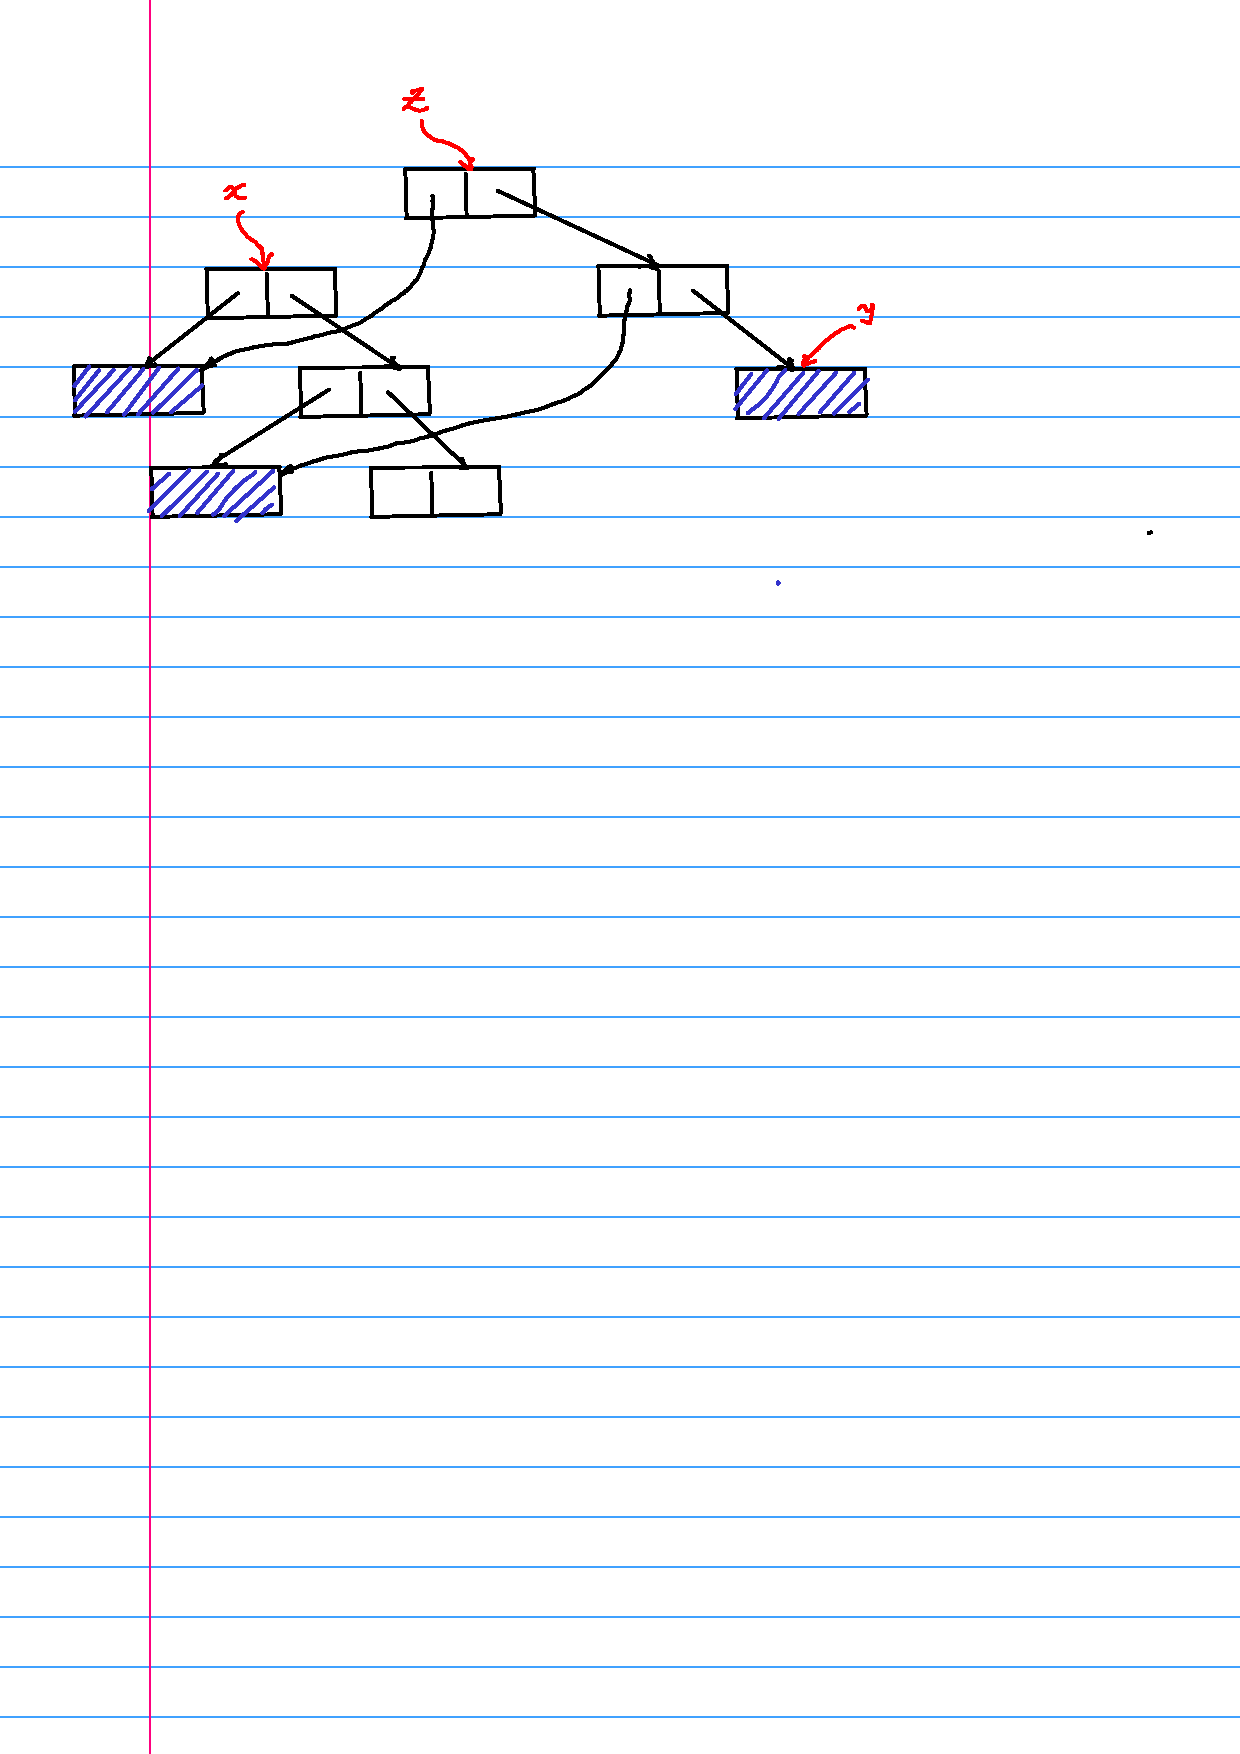
\includegraphics[width=.45\textwidth]{motiv-example}
      %%%%%%%%%%%%%%%%%%%%%Uday's stuff%%%%%%%%%%%%%%%%%%%%%%%%%
\psset{xunit=1mm, yunit=.8mm}
\psset{linewidth=.3mm}
\begin{pspicture}(0,17)(70,57)
%  \psframe(0,17)(70,57)
  %%%%%%%%%%%%%%%%%%%%%%%%%%%%%%%%%%%%%%%%%%%%%%%%%%%%%%%%%%%%%%%%
  \putnode{o}{origin}{13}{40}{\TwoCells{o1}{o2}}
  \putnode{a}{o}{-10}{-15}{\psframebox{5}}
  \ncline[offsetB=-.5,nodesepB=.1]{*->}{o1}{a}
  \putnode{y}{o}{-10}{10}{\psframebox[linestyle=none,framesep=.5]{$\px$}}
  \nccurve[nodesepB=-.2,angleA=330,angleB=120]{->}{y}{o}
  \aput[-2.5](.4){\scalebox{1.2}{\psframebox[framesep=.2,linestyle=none,fillstyle=solid,
	fillcolor=white]{$\times$}}}
  %%%%%%%%%%%%%%%%%%%%%%%%%%%%%%%%%%%%%%%%%%%%%%%%%%%%%%
  \putnode{c}{o}{25}{4}{\TwoCells{c1}{c2}}
  \putnode{d}{c}{10}{-10}{\TwoCellsAD{d1}{d2}}
  \putnode{e}{o}{10}{-15}{\TwoCellsAD{e1}{e2}}
  \putnode{f}{d}{13}{-12}{\TwoCellsAD{f1}{f2}}
  \ncline[nodesepB=-.5]{*->}{c2}{d}
  \ncline[nodesepB=-.5,linewidth=.7]{->}{c2}{d}
  \nccurve[ncurv=1,angleA=235,angleB=45]{*->}{c1}{a}
  \aput[-3.5](.2){\scalebox{1.2}{\psframebox[framesep=.2,linestyle=none,fillstyle=solid,
	fillcolor=white]{$\times$}}}
%  \putnode{g}{e}{-6}{-13}{\TwoCellsAD{g1}{g2}}
  \nccurve[nodesepB=-.5,angleA=240,angleB=30]{*->}{d1}{e}
  \aput[-2.5](.5){\scalebox{1.2}{\psframebox[framesep=.2,linestyle=none,fillstyle=solid,
	fillcolor=white]{$\times$}}}
  \ncline[angleA=300,angleB=110]{*->}{d2}{f}
  \ncline[angleA=300,angleB=110,linewidth=.7]{->}{d2}{f}
  \putnode{w}{c}{-8}{11}{\psframebox[linestyle=none,framesep=.2]{$\pz$}}
  \putnode{ww}{c}{30}{-5}{\psframebox[linestyle=none,framesep=.2]{$\py$}}
  \nccurve[nodesepB=-.2,angleA=330,angleB=120,linewidth=.7]{->}{w}{c}
  %%%%%%%%%%%%%%%%%%%%%%%%%%%%%%%%%%%%%%%%%%%%%%%%%%%%%%%%%%%%%%%%%%
  \ncline[offsetB=-.5,nodesepB=.1]{*->}{o2}{e}
  %\ncline[offsetB=-.1,nodesepB=-.2]{*->}{e1}{g}
  \nccurve[nodesepB=-.3,angleA=270,angleB=90,offsetB=.5]{->}{ww}{f}
  \aput[-3.5](.5){\scalebox{1.2}{\psframebox[framesep=.2,linestyle=none,
        fillstyle=solid, fillcolor=white]{$\times$}}}
  %%%%%%%%%%%%%%%%%%%%%%%%%%%%%%%%%%%%%%%%%%%%%%%%%%%%%%%%%%%%%%%%%%
\end{pspicture}
 \\ \\
      \renewcommand{\arraystretch}{.9}
      \begin{tabular}[t]{p{0.9\columnwidth}}
        (b) Memory graph at $\pi$.  \scalebox{.7}{\TwoCellsAD{a1}{a2}}
        denotes a closure. Thick edges denote live links. Traversal
        stops at edges marked $\times$ during garbage collection for
        a liveness-based collector.
      \end{tabular}
    \end{tabular} 
  \end{pspicture}
%  \vspace*{-3ex}
  \caption{Example Program and its Memory Graph}\label{fig:mot-example}
\end{figure}


Figure~\ref{fig:mot-example} shows an example program and the state of
the heap at  the program point $\pi$, i.e. just  before the evaluation
of $(\length\  \pz)$.  The heap is  represented by a graph  in which a
node either  represents atomic  values ($\NIL$,  integers etc.),  or a
\CONS\  cell  containing  $\CAR$  and  $\CDR$  fields,  or  a  closure
(represented  by  shaded  clouds).   Edges   in  the  graph  are  {\em
  references} and represent  variables  or fields.  The figure shows
the  lists \px\  and  \pz\ partially  evaluated.   The evaluation  was
triggered by the test (\NULLQ~(\CAR~\pz)) in the \SIF\ expression.


The edges  shown by thick  arrows are those  which are live  at $\pi$.
%% Only those  cell which have a future use  should be preserved
%% during garbage collection, all other
%% cells can be  reclaimed.
Thus if a garbage collection  takes place at
$\pi$ with the heap shown in Figure~\ref{fig:mot-example}(b), a
liveness-based collector (LGC) will preserve only the cells referenced
by  $\pz$,  and the live cells  constituting the  closure
referenced by $(\CDR~\pz)$.   In contrast, a reachability-based
collector (RGC) will preserve all cells.

In  this work  we show  that  static analysis  of heap  data can  help
garbage collectors in reclaiming more garbage.  The specific
contributions of this paper are
\begin{itemize}
\item  We  formulate  a  liveness  analysis for  a  lazy  first  order
  functional language and  prove its correctness. The correctness
  proof involves setting up a non-standard semantics as a
  specification of liveness and then proving that the analysis is
  correct with respect to the specification.   
\item Our  analysis results  in a set  of context-free  grammars along
  with  a fixed  set  of non-context-free  productions.  The  decision
  regarding  whether   to  copy  a  cell   during  garbage  collection
  translates  to the  membership problem  of such  grammars.  In  this
  paper, we  have shown the  undecidability of the  membership problem
  for  the  class  of  grammars  that result  from  our  analysis.  To
  circumvent the  problem, we  over-approximate the  grammars generated
  by the analysis with DFAs.
\item We  have implemented a garbage  collector that uses the  DFAs to
  retain live  cells.  Our  experiments reveal  interesting space-time
  trade-offs  in  the  engineering  of  the  collector---for  example,
  updating liveness  information carried in closures  during execution
  results  in   more  garbage  being  collected.    Empirical  results
  demonstrate the effectiveness of liveness-based garbage collection.
\end{itemize}
To the  best of our
  knowledge, this is the first work on liveness-based garbage
  collection      for      lazy     languages.       All      previous
  attempts~\cite{shaham01heap,   ran.shaham-sas03,   shaham02estimating,
    asati14lgc, karkare06effectiveness} have involved either
  imperative or  eager functional languages. 

\subsection{Organization of the paper}

\warning{Section~\ref{sec:defs}   introduces   the   syntax   of   the
  programming language  considered and gives a  small-step operational
  semantics for it.   The liveness analysis for this  language and its
  soundness   proof   is  presented   in   Section~\ref{sec:liveness}.
  Section~\ref{sec:computing} describes the formulation of liveness as
  grammars. We  also give a  proof of undecidability of  such grammars
  and    show    how   they    can    be    approximated   by    DFAs.
  Section~\ref{sec:GC-scheme}   discusses  details   of  the   garbage
  collector,  in  particular the  use  of  liveness DFAs  for  garbage
  collection.     We    report    our    experimental    results    in
  Section~\ref{sec:experiments}   along    with   some   observations.
  Section~\ref{sec:relatedwork}  discusses  previous work  related  to
  garbage  collection  and liveness  and  Section~\ref{sec:conclusion}
  discusses possible extensions and concludes the paper.}
\section{The target language---syntax and semantics}
\label{sec:defs}
Figure~\ref{fig:lang-syntax} describes the syntax  of our language. It
is a first order language with lazy semantics. Programs are restricted
to        be        in        Administrative        Normal        Form
(ANF)~\cite{chakravarty03perspective} where  all actual  parameters to
functions  are  variables.  While  this  restriction  does not  affect
expressibility,  this form  has  the benefit  of  making explicit  the
creation of  closures through  the $\LET$  construct.  \warning{ For
  now, we assume  $\LET$s  in our
language  are non-recursive;  in the  expression $\LET\,\,  x \leftarrow  s\,\,
\IN\,\, e$, $x$ should not occur in  $s$}. The  restriction of \LET\ to  a single
definition  is for  ease  of  exposition---generalization to  multiple
definitions does not add conceptual difficulties.  We further restrict
each variable in a program to  be distinct, so that no scope shadowing
occurs---this  simplifies  reasoning.  


The body  of a function ${\mathit  f}$ is denoted  as $e_{\mathit f}$.
 We assume that each program has a distinguished function
\mainpgm\      with      the      definition     $(\DEFINE\      ({\tt
  \mainpgm})\  e_\mainpgm)$ and  the execution  of the  program starts
with the call to \mainpgm.  We write $\pi\!:\!e$ to associate the label
$\pi$ (not  part of the language  syntax) with the  program point just
before expression $e$.

\begin{figure}[t]\footnotesize
\renewcommand{\arraystretch}{1}
\begin{eqnarray*}
   p \in \mathit{Prog} & \!\!\!::=\!\!\! & d_1 \ldots d_n \,\,\,\, e_\mainpgm
   \hspace{5em} \,\,\,\,\,\,\,\,\,\; \mbox{\em --- program}\\
    \mathit{df} \in Fdef & \!\!\!::=\!\!\! & (\DEFINE\,\, (f\,\, x_1 \,\, \ldots
\,\,x_n)\,\,
    e)
    \hspace{0.2em} \ \ \ \ \ \ \ \ \  \mbox{\em --- function def} \\
e \in \mathit{Expr} & \!\!\!::=\!\!\! &
\left\{\begin{array}{@{}ll@{\hspace{1em}}l}
       (\SIF\,\, x\,\, e_1\,\, e_2) && \!\!\!\mbox{\em --- conditional} \\
       (\LET\,\, x \leftarrow s\,\, \IN\,\, e) &&\!\!\! \mbox{\em --- let
binding} \\
       (\SRETURN\,\, x) && \!\!\!\mbox{\em --- return from function}
    \end{array}\right. \\
s \in \mathit{App} & \!\!\!::=\!\!\!  &
\left\{\begin{array}{@{}l@{\hspace{1.2em}}l}
       k & \mbox{\em --- constant (numeric or $\NIL$)}\\
       (\CONS\,\, x_1\,\, x_2) & \mbox{\em --- constructor} \\
       (\CAR\,\, x) & \\
       (\CDR\,\, x) & \mbox{\em --- selectors} \\
       (\NULLQ\,\, x) & \\
       (\PRIM\,\, x_1\,\, x_2) & \mbox{\em ---  tester/generic arithmetic} \\
%%       (\ID\,\, x) & \mbox{\em ---  identity function (for inlining)} \\
       (f\,\, x_1\,\,\ldots\,\, x_n) & \mbox{\em --- function application}
    \end{array}\right.
\end{eqnarray*}
  \caption{The syntax of our language}\label{fig:lang-syntax}
\figrule
\normalsize
\end{figure}


\begin{figure*}[t!]
%\comment{

\begin{center}\footnotesize
\renewcommand{\arraystretch}{1.5}
\begin{tabular}{|c|c|c|}
\hline
Premise & Transition & Rule name \\
\hline
\hline 
          & $\rho,\, (\rho', \ell, e)\!:\!S,\, \heap,\, \kappa
  \rightsquigarrow \rho',\, S,\, \heap[\ell := \kappa],\, e$    &  \sc{const}
\\
\hline
          & {$\rho, \,(\rho', \ell, e)\!:\!S,\, \heap,\, (\CONS~x~y)
\rightsquigarrow
$  $\rho',\, S,\, \heap[\ell := (\rho(x), \rho(y))],\, e$}     &  \sc{cons} \\
\hline

$\heap(\rho(x)) \mbox{ is } (v, d)$ & $\rho,\, (\rho', \ell, e)\!:\!S,\, \heap,\,
(\CAR~x)  \rightsquigarrow \rho',\, S,\, \heap[\ell := v],\, e$      &
\sc{car-select} \\
\hline



$\heap(\rho(x)) \mbox{ is } (\langle s, \rho'\rangle, d)$ & $\rho,\, S,\,  \heap,\,
(\CAR~x)  \rightsquigarrow \rho', \,(\rho, addr(\langle s, \rho'\rangle), (\CAR~x))\!:\!S,\, \heap,\, s$      &
\sc{car-1-clo} \\
\hline

$\heap(\rho(x)) \mbox{ is } \langle s, \rho'\rangle$ & $\rho,\, S,\, \heap,\, (\CAR~x)
\rightsquigarrow
\rho',\, (\rho, \rho(x), (\CAR~x))\!:\!S, \,\heap,\, s$      &
\sc{car-clo}
\\
\hline



$\heap(\rho(x)), \heap(\rho(y)) \in \mathbb{N}$
 & {$\rho,\, (\rho', \ell, e)\!:\!S,\, \heap,\, (+~x~y)  \rightsquigarrow$
$\rho', \,S,\, \heap[\ell := \heap(\rho'(x)) + \heap(\rho'(y))],\, e$}      &
\sc{prim-add} \\
\hline

$\heap(\rho(x)) \mbox{ is } \langle s, \rho'\rangle$ & $\rho,\, S,\, \heap,\, (+~x~y)
\rightsquigarrow
\rho',\, (\rho, \rho(x), (+~x~y))\!:\!S,\, \heap,\, s$      &
\sc{prim-1-clo} \\
\hline
$\heap(\rho(y)) \mbox{ is } \langle s, \rho'\rangle $ & $\rho,\, S,\, \heap,\, (+~x~y)
\rightsquigarrow
\rho', (\rho,\, \rho(y),\, (+~x~y))\!:\!S,\, \heap,\, s$      &
\sc{prim-2-clo} \\
\hline
{$\mathit{f}~\mbox{defined as}$
$~(\DEFINE~(f~\myvec{y})~e_{\mathit{f}})$}  & $\rho,\, S,\, \heap,\,
(f~\myvec{x})  \rightsquigarrow
[\myvec{y} \mapsto \rho(\myvec{x})],\, S,\, \heap,\, e_{\mathit{f}}$      &
\sc{funcall} \\
\hline
$\ell$ is a new location& {$\rho,\, S,\, \heap,\, (\LET~x\leftarrow s~\IN~e)
  \rightsquigarrow$
$\rho\oplus[x \mapsto \ell],\, S,\, \heap[\ell \mapsto \langle s,
    \lfloor\rho\rfloor_{FV(s)} %% \oplus [x \mapsto  \ell] -- NO LAZY LETS
    \rangle],\, e$} &
\sc{let} \\
\hline
$\heap(\rho(x)) \ne 0$ & $\rho,\, S,\, \heap,\, (\SIF~x~e_1~e_2)   \rightsquigarrow
\rho,\, S,\, \heap,\,  e_1$ & \sc{if-true} \\
\hline
$\heap(\rho(x)) = 0$ & $\rho,\, S,\, \heap,\, (\SIF~x~e_1~e_2)   \rightsquigarrow
\rho,\, S, \,\heap, \, e_2$ & \sc{if-false} \\
\hline
$\heap(\rho(x)) = \langle s, \rho' \rangle $ & {$\rho,\, S,\, \heap,\,
  (\SIF~x~e_1~e_2)   \rightsquigarrow
\rho',\, (\rho, \rho(x), (\SIF~x~e_1~e_2))\!:\!S,\, \heap, \, s$}
&
\sc{if-clo} \\
\hline
{$\heap(\rho(x))~\mbox{is in WHNF with value}~v$}& $\rho,\, (\rho', \ell,
e)\!:\!S,\, \heap,\,
(\SRETURN~x)  \rightsquigarrow \rho',\, S,\, \heap[\ell := v],\, e$ &
\sc{return-whnf}\\
\hline
$\heap(\rho(x)) = \langle s, \rho' \rangle $ & {$\rho,\, S,\, \heap,\, (\SRETURN~x)
  \rightsquigarrow$
$\rho',\, (\rho, \rho(x), (\SRETURN~x))\!:\!S,\, \heap,\,  s$} &
\sc{return-clo} \\
\hline
\end{tabular}
\caption{The small-step semantics for the language. \label{fig:lang-semantics}}
\end{center}
%}\comment
\end{figure*}



\subsection{Semantics}
%\comment{
We now give  a small-step semantics for our  language.
We first specify the domains used by the semantics:
\[
\renewcommand{\arraystretch}{1}
\begin{array}{@{}r@{\ }l@{\ \ }c@{\ \ }l@{\hspace{0.5em}}l}
\heap: & \mathit{Heap} & =&\mathit{Loc} \rightarrow (Data + \{empty\}) & \mbox{-- Heap}\\
d: & \mathit{Data} &=&\mathit{Val} + \mathit{Clo} & \mbox{-- Values \& Closures} \\
v:   & \mathit{Val} &=& \mathbb{N} + \{\NIL\} + \mathit{Data \times Data}& \mbox{-- Values}\\
c:   & \mathit{Clo} &=& \mathit{(App \times Env)}& \mbox{-- Closures}\\
\rho: & \mathit{Env} &=&\mathit{Var} \rightarrow \mathit{Loc} &
\mbox{-- Environment} \\
\end{array}
\]


Here  $\mathit{Loc}$ is  a countable  set  of locations  in the  heap.
A non-empty location either contains  a value in  \emph{WHNF} (a  number, the
empty  list  $\NIL$ or  a  \CONS\  cell  with  possibly  unevaluated
constituents) or  a {\em closure}.   A closure  is a pair  $\langle s,
\rho\rangle$ in  which $s$ is  an unevaluated application,  and $\rho$
maps free variables of $s$ to their respective locations. Since all data objects are boxed, we model an environment as a mapping
from the set  of variables of the program  $\mathit{Var}$ to locations
in the  heap.  


The  semantics  of   expressions  (and  applications)
%% \footnote{In  most
%%   contexts, we  shall use the  term 'expression' and the  notation $e$
%%   for both expressions and applications.} 
are given by transitions of
the form $\rho, \stk, \heap,  e \rightarrow \rho', \stk', \heap', e'$.
Here \stk\ is a stack of continuation frames.  Each continuation frame
is of the form $(\rho, \ell,  e)$, signifying that the location $\ell$
has  to  be  updated  with  the  value  of  the  currently  evaluating
expression, and $e$ is to be evaluated next in the environment $\rho$.
Note  that  the  state  of  the  transition  system  consists  of  the
\emph{current evaluation  context}, given by  $\rho$ and $e$,  and the
\emph{suspended  evaluation  contexts}  (represented  as  continuation
frames) in the stack $S$.   
%% \warning{The
%% 3-tuple $\rho, \stk,  \heap, e$ representing the state  of the transition
%% system will be denoted $\mathcal{S}$.}

The  initial  state  of  the  transition  system  described  above  is
$([\;]_\rho,\,   (\rho_\mathit{init},   \, \ell_{\ans}  ,\,
(\print~\ans)):[\;]_{S}, 
[\;]_{\heap},\, (\mainpgm))$,  in which  $[\;]_\rho$,
$[\;]_{\mbox \footnotesize {H}}$
and $[\;]_{S}$ are    are the
empty environment, heap and stack respectively. The  initial stack consists
of  a single  continuation frame  in  which \ans\  is a  distinguished
variable  that  would   eventually  be  updated  with   the  value  of
(\mainpgm) and $\rho_\mathit{init}$ maps \ans\ to a location $\ell_{\ans}$.   In  addition, \print\ is  a function modeling  a printing
mechanism---a   standard   run-time   support  assumption   for   lazy
languages~\cite{Jones87}---that prints  the value of  (\mainpgm).  The operator $:$
pushes elements on top of the stack.

The   notation  $[\myvec{x}   \mapsto  \myvec{\ell}]$   represents  an
environment  that  maps  variables  $x_i$ to  locations  $\ell_i$  and
$\heap[\ell := d]$  indicates the updating of a heap  \heap\ at $\ell$
with  $d$.   $\rho \oplus  \rho'$  represents  the environment  $\rho$
shadowed  by  $\rho'$  and  $\lfloor \rho  \rfloor_X$  represents  the
environment  restricted  to  the  variables in  $X$.  Finally  $FV(s)$
represents the  free variables  in the  application $s$  and $addr(c)$
gives the address of the closure $c$ in the heap.

The small-step semantics  is shown in Figure~\ref{fig:lang-semantics}.
Unlike   an   eager  language,   evaluation   of   a  let   expression
$(\LET~x\leftarrow  s~\IN~e)$ does  not  result in  the evaluation  of
$s$. Instead,  as the {\sc let}  rule shows, a closure  is created and
bound to  $x$. The  program points which  trigger evaluation  of these
closure   are  the   condition  of   an  $\SIF$   ({\sc  IF-clo})   and
\SRETURN\ ({\sc  return-clo}).  We  call such  points \emph{evaluation
  points   $(\epath)$}  and   label  them   with  $\psi$   instead  of
$\pi$. As an  example of closure  evaluation, we  explain the
three rules for  $(\CAR~x)$.  If $x$ is a closure,  it is evaluated to
WHNF, say $(d_1, d_2)$.  This is  given by the rule {\sc car-clo}.  If
$d_1$ is  not in WHNF,  it is  also evaluated ({\sc  car-1-clo}).  The
address  to be  updated  with the  evaluated value  is
recorded  in  a  continuation  frame.    This  is  required  for  lazy
evaluation, else $d_1$ may  be evaluated more than once
due to  sharing~\cite{Jones87}.  Only after this  is the actual selection  done ({\sc
  car-select}).


%}\comment
%==============================================================
\renewcommand{\pp}[2]{\ensuremath{#1\!\!:\!#2}} % prog point
%==============================================================
\begin{figure}[t!]
  \renewcommand{\arraystretch}{1.4}
  \small
\hspace*{-6pt}
$\begin{array}{@{}r@{\ }c@{\ }l@{}}
\mathit{ref\/}(\kappa,\sigma,\Lfonly) &=& \emptyset \mbox{, for $\kappa$ a constant, including \NIL} \\

\mathit{ref\/}(\pp{\pi}{(\CONS~x~y)},\sigma,\Lfonly)
&=& \{x_{\pi}.\alpha \mid \acar\alpha \in \sigma\} \cup
\{y_{\pi}.\alpha 
\mid \acdr\alpha \in \sigma\} \\

\mathit{ref\/}(\pp{\pi}{(\CAR~x)},\sigma,\Lfonly)
&=&\!\left\{\!\!\!\!\begin{array}{l@{\ }l}
  \{x_{\pi}.\epsilon\} \cup \{x_{\pi}.\acar\alpha \mid \alpha \in
  \sigma\}, & \mbox{if}~\sigma \ne \emptyset\\
  \emptyset  & \mbox{otherwise}
\end{array}\right. \\

\mathit{ref\/}(\pp{\pi}{(\CDR~x)},\sigma,\Lfonly)
&=&\!\left\{\!\!\!\!\begin{array}{l@{\ }l}
\{x_{\pi}.\epsilon\} \cup \{x_{\pi}.\acdr\alpha \mid \alpha \in
\sigma\}, & \mbox{if}~\sigma \ne \emptyset\\
\emptyset  & \mbox{otherwise}
\end{array}\right. \\

\mathit{ref\/}(\pp{\pi}{(\PRIM~x~y)},\sigma,\Lfonly)
&=&\!\left\{\!\!\!\!\begin{array}{l@{\ }l}
\{x_{\pi}.\epsilon, y_{\pi}.\epsilon\},  & \mbox{if}~\sigma \ne
\emptyset\\
\emptyset  & \mbox{otherwise}
\end{array}\right.\\

\mathit{ref\/}(\pp{\pi}{(\NULLQ~x)},\sigma,\Lfonly)
&=&\!\left\{\!\!\!\!\begin{array}{l@{\ }l}
\{x_{\pi}.\epsilon\},  & \mbox{if}~\sigma \ne \emptyset\\
\emptyset  & \mbox{otherwise}
\end{array}\right. \\

\mathit{ref\/}(\pp{\pi}{(f~\myvec{x})},\sigma,\Lfonly)
%          &=& \bigcup_{i=1}^n y_i.\Lf{f}{i}{\sigma}
&=&  \begin{array}{@{}l}  % to discourage \displaystyle
  \bigcup_{i=1}^n x_{i_{\pi}}.\Lf{f}{i}{\sigma}
\end{array}
%          &=& \bigcup \{y_i.\Lf{f}{i}{\sigma} \mid i=1,\ldots, n\}
\\

\mathcal{L}((\SRETURN~\pp{\psi\ }{x}),\sigma,\Lfonly) &=& 
x.\sigma\\

\mathcal{L}((\SIF~\pp{\psi\ }{x~e_1~e_2}),\sigma,\Lfonly) &=&
\!\left\{\!\!\!\!\begin{array}{l@{\ }l}
  \mathcal{L}(e_1,\sigma,\Lfonly) \cup
  \mathcal{L}(e_2,\sigma,\Lfonly) \cup
  \{x.\epsilon\},  & \\ 
  \qquad\qquad\qquad\qquad\qquad\qquad\mbox{if}~\sigma \ne \emptyset & \\
  \emptyset  \qquad\qquad\qquad\qquad\qquad\quad\; \mbox{otherwise} &\\
\end{array}\right. \\

\mathcal{L}((\LET~x \leftarrow~s~\IN~e),\sigma,\Lfonly) &=&
\mathit{ref\/}(s,\sigma',\Lfonly) \cup \Lv \cup \{x.\sigma'\} 
\\
&&~\mbox{where}~ \mathcal{\Lv} = \mathcal{L}(e,\sigma,\Lfonly),\\
&&~\mbox{and}~\sigma' = \bigcup_{\pi}  \Lv(x_{\pi})
\\ & \\
\end{array}$
\begin{center}
\begin{minipage}{0.95\columnwidth}

  \infrule[live-define]
          {\mathcal{L}(e_f,\sigma,\Lfonly) =
            \bigcup_{i=1}^n z_i.\Lf{f}{i}{\sigma}
            \mbox{ for each $f$ and $\sigma$}
          }
          { \mathit{df_1} \ldots \mathit{df_k} \len \Lfonly
            \\ \makebox[20mm]{\rule{15mm}{0pt}where
              $(\DEFINE\ (f\ z_1\ \ldots\ z_n)\ \ e_f)$ 
              is a member of $\mathit{df_1}
              \ldots \mathit{df_k}$}}
\end{minipage}
\end{center}
\caption{Liveness equations and judgement rule}\label{fig:live-judge}
\vspace*{-12pt}
\end{figure}



\section{Liveness}
\label{sec:liveness}

A variable is {\em live} if there  is a possibility of its value being
used in  future computations and  dead if  it is definitely  not used.
Heap-allocated data  needs a richer model  than classical liveness---a
model  which  talks  about  liveness of  references.   Using  $\acar$,
$\acdr$  to  represent access  using  $\CAR$  and $\CDR$  fields,  the
liveness of the structure reachable from a variable can be represented
by a set of {\em access paths} i.e.  prefix-closed set of strings from
$\{\acar,\acdr\}^\ast$.  Given an initial location $\ell$ (typically a
variable  reference) and  a heap  \heap, semantically  an access  path
$\alpha$ represents  a reference, denoted $\heap\oxlb\ell,  \alpha\oxrb$, in
the heap  that is  obtained by  starting with  $\ell$ and  chasing the
\CAR\ or  \CDR\ fields  as specified  by the  access path.  
$\heap\oxlb\ell, \alpha\oxrb$  is defined only  if the path followed  in the
heap  is \emph{closure-free}  (does not  cross closures),  else it  is
undefined.

Access paths can be used to  represent liveness. As an example, if $x$
is  a  list  with  liveness  $\{\epsilon,  \acar,  \acdr,  \acdr\acar,
\acdr\acdr,  \acdr\acdr\acar\}$,  then  future computations  can  only
refer up  to the  second and  third members of  $x$.  A  {\em liveness
  environment} is a mapping from  variables to access paths, but often
expressed as  a set,  for example  by writing  $\{x.\epsilon, x.\acdr,
x.\acdr\acdr,        y.\epsilon\}$        instead        of        $[x
  \mapsto\{\epsilon,\acdr,\acdr\acdr\},          y\mapsto\{\epsilon\},
  z\mapsto\{\}]$.    In  this   notation,  $y   \mapsto  \{\epsilon\}$
represents access using $y$ itself and $z \mapsto \{\}$ indicates that
$z$ is dead.  In lazy  languages, liveness environments are associated
with regions of programs instead of program points.

A notion  that generalizes liveness  is {\em demand}.   While liveness
gives the patterns of future uses of a variable, demand represents the
future use of the value of an expression.  The demand on an expression
$e$   is   again   a   set    of   access   paths---that   subset   of
$\{\acar,\acdr\}^\ast$ which the  context of $e$ may  explore of $e$'s
result.   To see  the need  for demands,  consider the  let expression
$(\LET~x\leftarrow  (\CDR~y)~\IN~   \SRETURN~x)$.   Assume   that  the
context of this expression places  the demand $\lbrace \epsilon, \acar
\rbrace$. Since the  value of the expression is the  value of $x$, the
demand translates to the liveness  $[x \mapsto \lbrace \epsilon, \acar
  \rbrace]$.   Due  to  the  \LET\   definition  which  binds  $x$  to
$(\CDR~y)$, the liveness of $x$  now becomes the demand on $(\CDR~y)$.
This, in  turn, generates  the liveness $\lbrace  y.\epsilon, y.\acdr,
y.\acdr\acar  \rbrace$.   These are  the  set  of $y$-rooted  accesses
required to  explore $\lbrace  \epsilon, \acar  \rbrace$ paths  of the
result of $(\CDR~y)$.
%% As an  analogy with classical  (strong) liveness analysis,  $y$ and
%% $z$ are live at the entry $\pi: x:=y+z$, if and only if $x$ is live
%% at  exit  of $\pi$.   In  our  terminology, the  liveness  $\lbrace
%% \epsilon\rbrace $ of $x$ at the  exit from $\pi$ becomes the demand
%% on  $y+z$,  and  this,  in turn  generates  the  liveness  $\lbrace
%% y.\epsilon, z.\epsilon \rbrace$ at the entry of $\pi$.

We use $\sigma$  to range over demands, $\alpha$ to  range over access
paths  and $\Lv$  to range  over liveness  environments. $\Lv_y$  will
denote  the liveness  of an  individual  variable $y$  in $\Lv$.   The
notation $\sigma_1\sigma_2$ denotes  the set $\lbrace \alpha_1\alpha_2
\mid \alpha_1  \in \sigma_1, \alpha_2 \in  \sigma_2\rbrace$.  Often we
shall abuse  notation to juxtapose an  edge label and a  set of access
paths; $\acar\sigma$ is a shorthand for $\lbrace\acar\rbrace\sigma$.

%% \begin{figure*}[t!]
%% \renewcommand{\arraystretch}{1}
%%   \begin{tabular}{cc}
%%     \begin{minipage}{.40\textwidth}
%%         \small
%%         \renewcommand{\arraystretch}{1}{
%%           \begin{uprogram}
%%             \UNL{1} (\DEFINE\ (\length~\xl)
%%             \UNL{2}  $\pi_1\!\!:\, $(\LET\ \px\ $\leftarrow $\
%% (\NULLQ~\xl) \IN
%%             \UNL{3} \hspace*{.05cm} $\pi_2\!\!:\,$(\SIF\
%% $\psi_1\!\!:\,$ \px
%%             \UNL{4} \hspace*{.27cm} $\pi_3\!\!:\,
%%             $(\LET\ \pv\ $\leftarrow 0$ \IN
%%             \UNL{5} \hspace*{.32cm} $\pi_4\!\!:\,
%% (\SRETURN~\psi_2:\pv)$
%%             \UNL{4} \hspace*{.29cm}    $\pi_5\!\!:\, $(\LET~\pu\
%% $\leftarrow$  (\CDR~\xl)  \IN
%%             \UNL{5} \hspace*{.34cm}   $\pi_6\!\!:\, $(\LET~\py\
%% $\leftarrow$  (\length~\pu)  \IN
%%             \UNL{6} \hspace*{.34cm} $\pi_7\!\!:\,
%%             $(\LET~\pz\ $\leftarrow$ (1~+~\py) \IN
%%             \UNL{7} \hspace*{.34cm} $\pi_8\!\!:\,
%% (\SRETURN~\psi_3:\pz)$)))))))
%%         \end{uprogram}}
%%         \renewcommand{\arraystretch}{1}{
%% 	  \begin{uprogram}
%% 	  \UNL{1} $(\DEFINE\ (\main)$
%%            \UNL{2} \!\!$\pi_9\!\!:\, (\LET\  \pa\  \leftarrow$
%%            (
%%            \scalebox{0.8}{\psframebox[framearc=.5,
%% 	fillcolor=lightgray,fillstyle=solid,framesep=2pt]{%
%%              \begin{tabular}{@{}c@{}}
%%                {a BIG closure}
%%              \end{tabular}}}
%%            ) \IN  
%%           \UNL{3} \!\!$\pi_{10}\!\!:\, (\LET\  \pb\  \leftarrow ($+$\ \pa\ \acdr)$
%% \IN
%% 	  \UNL{4}   \hspace*{.05cm}$\pi_{11}\!\!:\,      $ (\LET\ \pc\
%% $\leftarrow  (\CONS\ \pb\ \NIL)$ \IN
%%           \UNL{5}   \hspace*{.15cm}    $\pi_{12}\!\!:\,
%%           $(\LET\ \pw\  $\leftarrow  (\length\ \pc)$ \IN
%%           \UNL{6}  \hspace*{.25cm}  $\pi_{13}\!\!:\,
%% (\SRETURN~\psi_4:\pw)))))$
%% \end{uprogram}}
%%         %%}
%%     \end{minipage}

%%     &

%%     \begin{minipage}{.51\textwidth}

%%       \small
%% \begin{eqnarray*}
%%         \mathcal{L}(e_{\length},\sigma,\Lfonly) &=&
%%               [\;\epath_1 \mapsto \lbrace \px.\clazy \sigma,
%% \xl.\clazy\sigma\rbrace ,~\epath_2 \mapsto \lbrace 
%% \pv.\sigma  \rbrace,\\
%%  &&          \;\;  \epath_3 \mapsto \lbrace \pz.\sigma,
%%                 \py.\clazy\sigma,
%% \pu.\Lf{\length}{\mbox{1}}{\clazy\sigma},\\
%% &&            \;\;\;\;\;\;\;\;\;\;\;\;\;\;\;\;\;
%% \xl.\{ \acdr\Lf{\length}{\mbox{1}}{\clazy\sigma} \cup
%% %%\;\;\;\;\;\;\; \;\;\;\;\;\;\;\;\;\;\;\;\;\;\;\;\\
%% \clazy\Lf{\length}{1}{\clazy\sigma}\}\}
%%              \rbrack \\
%%             \cal{P_{\mbox{\tiny \length}}} &=&
%%                 [\;\pi_1 \mapsto \lbrace \epath_1, \epath_2, \epath_3 \rbrace,  \
%%                  \pi_2 \mapsto \lbrace \epath_1, \epath_2, \epath_3
%%                   \rbrace, \\
%% &&\;\;  \pi_3 \mapsto \lbrace \epath_2
%%                   \rbrace ,  \pi_4 \mapsto \lbrace \epath_2
%%                   \rbrace, \pi_5 \mapsto \lbrace  \epath_3 \rbrace, \\
%%  &&  \;\;                        \pi_6 \mapsto \lbrace \epath_3 \rbrace,
%% \pi_7 \mapsto
%%                    \lbrace \epath_3\rbrace, \pi_8 \mapsto \lbrace \epath_3
%% \rbrace~\rbrack\\
%%               \mathcal{L}(e_{\main},\sigma,\Lfonly) &=&
%%                 [\;
%%                   \epath_4 \mapsto \lbrace \pw.\sigma,
%%                                        \pc.\Lf{\length}{\mbox{1}}{\sigma},\\
%% && \;\;\;\;\;\;\;\;\;\;\;\;\;\;\;\;\;\;
%% \pb.\bcar\Lf{\length}{\mbox{1}}{\sigma},
%% \pa.\clazy\bcar\Lf{\length}{\mbox{1}}{\sigma} \rbrace
%%                                ] \\
%%                \cal{P_{\mbox{\tiny \main}}} &=&
%%                   \lbrack~ \pi_9 \mapsto \lbrace \epath_4 \rbrace,  \
%%                     \pi_{10} \mapsto \lbrace \epath_4 \rbrace,  \
%%                    \pi_{11} \mapsto \lbrace \epath_4 \rbrace, \\
%%                    && \;\; \pi_{12} \mapsto \lbrace \epath_4 \rbrace,
%% \pi_{13} \mapsto \lbrace \epath_4 \rbrace~\rbrack
%% \end{eqnarray*}
%%     \end{minipage} \\
%% (a)&
%% (b)
%%     %% \end{ tabular}}
%%   \end{tabular}
%% %\end{picture}
%% \kern -3ex
%% %\vspace{0.5in}
%% \caption{(a) Example program and (b) its liveness
%% maps.}\label{fig:mot-example2}
%% \end{figure*}
%% %================================================================

\begin{figure*}[t!]
\renewcommand{\arraystretch}{1}
  \begin{tabular}{cc}
    \begin{minipage}{.50\textwidth}
        \small
        \renewcommand{\arraystretch}{1}{
          \begin{uprogram}
            \UNL{1} (\DEFINE\ (\fun~\px\ \pn)
            \UNL{2}  $\pi_1\!\!:\, $(\LET\ \py\ $\leftarrow $\
(\length~\px) \IN
            \UNL{3} $\pi_2\!\!:\, $(\LET\ \pl\ $\leftarrow $\
(\makelist~\pn) \IN
            \UNL{4} \hspace*{.05cm} $\pi_3\!\!:\,$(\SIF\
$\psi_1\!\!:\,$ \py
            \UNL{5} \hspace*{.27cm} $\pi_4\!\!:\, $(\LET\ \xhd\ $\leftarrow$\ (\CAR\ \pl) \IN
            \UNL{6} \hspace*{.27cm} $\pi_5\!\!:\, $(\LET\ \xtl\ $\leftarrow$\ (\CDR\ \px) \IN
            \UNL{7} \hspace*{.27cm} $\pi_6\!\!:\, $(\LET\ \rest\ $\leftarrow$\ (\fun~ \xtl\ \xhd) \IN
            \UNL{8} \hspace*{.27cm} $\pi_7\!\!:\, $(\LET\ \ret\ $\leftarrow$\ (\CONS\ \py\ \rest) \IN
            \UNL{9} \hspace*{.32cm} $\pi_8\!\!:\,
(\SRETURN~\psi_2:\ret)))))$
            \UNL{5} \hspace*{.29cm}    $\pi_9\!\!:\, $(\LET~\ps\
$\leftarrow$  (\Sum~\pl)  \IN
            \UNL{6} \hspace*{.34cm}   $\pi_{10}\!\!:\, $(\LET~\pu\
$\leftarrow$  (+~1~\py)  \IN
            \UNL{7} \hspace*{.34cm} $\pi_{11}\!\!:\,
            $(\LET~\pr\ $\leftarrow$ ($/$~\ps~\pu) \IN
            \UNL{8} \hspace*{.27cm} $\pi_{12}\!\!:\, $(\LET\ \res\ $\leftarrow$\ (\CONS\ \pr\ \NIL) \IN
            \UNL{9} \hspace*{.34cm} $\pi_{13}\!\!:\,
(\SRETURN~\psi_3:\res)$)))))))))
        \end{uprogram}}
        \renewcommand{\arraystretch}{1}{
	  \begin{uprogram}
	  \UNL{1} $(\DEFINE\ (\main)$
           \UNL{2} \!\!$\pi_{14}\!\!:\, (\LET\  \pa\  \leftarrow$
           (\CONS\ $1$\ (\CONS\ $2$\ \NIL) \IN  
          \UNL{3} \!\!$\pi_{15}\!\!:\, (\LET\  \pb\  \leftarrow $5$)$
\IN
	  \UNL{4}   \hspace*{.05cm}$\pi_{16}\!\!:\,      $ (\LET\ \pc\
$\leftarrow  (\fun\ \pa\ \pb)$ \IN
          \UNL{5}   \hspace*{.15cm}    $\pi_{17}\!\!:\,
          (\SRETURN~\psi_4:\pc)))))$
\end{uprogram}}
        %%}
    \end{minipage}

    &

    \begin{minipage}{.48\textwidth}

      \small
\begin{eqnarray*}
        \mathcal{L}(e_{\length},\sigma,\Lfonly) &=&
              [\;\epath_1 \mapsto \lbrace \px.\clazy \sigma,
\xl.\clazy\sigma\rbrace ,~\epath_2 \mapsto \lbrace 
\pv.\sigma  \rbrace,\\
 &&          \;\;  \epath_3 \mapsto \lbrace \pz.\sigma,
                \py.\clazy\sigma,
\pu.\Lf{\length}{\mbox{1}}{\clazy\sigma},\\
&&            \;\;\;\;\;\;\;\;\;\;\;\;\;\;\;\;\;
\xl.\{ \acdr\Lf{\length}{\mbox{1}}{\clazy\sigma} \cup
%%\;\;\;\;\;\;\; \;\;\;\;\;\;\;\;\;\;\;\;\;\;\;\;\\
\clazy\Lf{\length}{1}{\clazy\sigma}\}\}
             \rbrack \\
            \cal{P_{\mbox{\tiny \length}}} &=&
                [\;\pi_1 \mapsto \lbrace \epath_1, \epath_2, \epath_3 \rbrace,  \
                 \pi_2 \mapsto \lbrace \epath_1, \epath_2, \epath_3
                  \rbrace, \\
&&\;\;  \pi_3 \mapsto \lbrace \epath_2
                  \rbrace ,  \pi_4 \mapsto \lbrace \epath_2
                  \rbrace, \pi_5 \mapsto \lbrace  \epath_3 \rbrace, \\
 &&  \;\;                        \pi_6 \mapsto \lbrace \epath_3 \rbrace,
\pi_7 \mapsto
                   \lbrace \epath_3\rbrace, \pi_8 \mapsto \lbrace \epath_3
\rbrace~\rbrack\\
              \mathcal{L}(e_{\main},\sigma,\Lfonly) &=&
                [\;
                  \epath_4 \mapsto \lbrace \pw.\sigma,
                                       \pc.\Lf{\length}{\mbox{1}}{\sigma},\\
&& \;\;\;\;\;\;\;\;\;\;\;\;\;\;\;\;\;\;
\pb.\bcar\Lf{\length}{\mbox{1}}{\sigma},
\pa.\clazy\bcar\Lf{\length}{\mbox{1}}{\sigma} \rbrace
                               ] \\
               \cal{P_{\mbox{\tiny \main}}} &=&
                  \lbrack~ \pi_9 \mapsto \lbrace \epath_4 \rbrace,  \
                    \pi_{10} \mapsto \lbrace \epath_4 \rbrace,  \
                   \pi_{11} \mapsto \lbrace \epath_4 \rbrace, \\
                   && \;\; \pi_{12} \mapsto \lbrace \epath_4 \rbrace,
\pi_{13} \mapsto \lbrace \epath_4 \rbrace~\rbrack
\end{eqnarray*}
    \end{minipage} \\
(a)&
(b)
    %% \end{ tabular}}
  \end{tabular}
%\end{picture}
\kern -3ex
%\vspace{0.5in}
\caption{(a) Example program and (b) its liveness
maps.}\label{fig:mot-example2}
\end{figure*}
%================================================================

%%\label{fig:mot-example2}

\subsection{Liveness Analysis for lazy languages}
\label{sec:liveness-analysis}
 
%\comment{ 
Consider  the program in  Figure~\ref{fig:mot-example2}.  As
  mentioned earlier,  a lazy  evaluation of  the $\LET$  expression at
  $\pi_1$ creates a closure for $(length~x)$ instead of evaluating it.
  Since the  closure may escape the  scope in which it  is created, it
  carries a copy  of $x$ within itself.   We treat the copy  of $x$ in
  the closure as being separate from the $x$ introduced by the $\LET$,
  and call  it a \emph{closure variable}.   For liveness calculations,
  such variables are distinguished from variables introduced by \LET s
  and  function arguments  (called \emph{stack  variables} since  they
  reside in the activation stack). Notationally, we distinguish
  closure variables from their corresponding stack variables by
  subscripting them with their program points of
  creation.\footnote{Mutiple occurrences of the same variable in an
    application are further distinguished by their positions in the
    application.}


  Since a  closure is evaluated  only at evaluation points,  a closure
  variable is attributed  with the same liveness in the  region of the
  program from the  point of creation to  reachable evaluation points.
  This is  also true  of stack  variables, because,  as we  shall see,
  stack variables derive their  liveness from closure variables. Thus,
  there are  two major differences  in our formulation of  liveness of
  lazy   languages  with   liveness  of   eager 
  languages~\cite{asati14lgc}:    (i)  the
  introduction of  closure variables in the  liveness calculation, and
  (ii) a  single liveness value  for each variable that  is applicable
  from its creation point to evaluation points.


  Closure  variables get  their  liveness values  through  a chain  of
  dependences beginning at  a variable at an evaluation  point.  As an
  example,  the  variable $z$  returned  at  $\psi_2$ depends  on  $y$
  through  the  expression $(+~y~1)$.   $y$  in  turn depends  on  the
  closure  variable  $x_{\pi_1}$   through  $(length~x_{\pi_1})$.   We
  denote  this chain  of dependences  as $\lbrack  \psi_2\!\!\!:\!\!\!z \leftarrow
  (+~y~1),\,  y  \leftarrow   (length~x_{\pi_1})\rbrack$.   Indeed,  the
  closures  in  the  heap  are   a  runtime  representation  of  these
  dependences.  Since  $z$  is  evaluated   at  $\psi_2$  due  to  the
  expression $\SRETURN~z$,  the demand made by  the calling context(s)
  of  $f$ places  a demand  on  $z$ which  will impart  a liveness  to
  $x_{\pi_1}$.  Other dependence chains which result in a liveness for
  $x_{\pi_1}$       are       $\lbrack       \psi_1\!\!\!:\!\!y       \leftarrow
  (length~x_{\pi_1})\rbrack$ and $\lbrack \psi_3\!\!\!:\!\!\!w \leftarrow (/~u~y),\,\,
  y  \leftarrow  (length~x_{\pi_1})\rbrack$.   The  liveness  analysis
  described in this section declares the liveness of $x_{\pi_1}$ to be
  a union of the liveness arising  out of these dependence chains.  To
  be safe, a  garbage collection during evaluation of  $y$ at $\psi_1$
  has  to  use  this  liveness  to copy  the  heap  from  $x_{\pi_1}$.
  However,  notice that  if  a garbage  collection  takes place  while
  evaluating $z$ at $\psi_2$, it can safely consider only the liveness
  arising  out of  the dependence  chain\linebreak $\lbrack  \psi_2\!\!\!:\!\!\!z \leftarrow
  (y+1),\,   y  \leftarrow   (length~x_{\pi_1})\rbrack$.   The   garbage
  collection  scheme described  in Section~\ref{sec:GC-scheme}  uses a
  generalization  of   this  observation   to  dynamically   select  a
  evaluation point specific liveness in order to collect more garbage.



Figure~\ref{fig:live-judge}  describes  our  analysis  which  has  two
parts. The  function $\mathit{ref}$,  takes an  application $s$  and a
demand $\sigma$ and returns the incremental liveness generated for the
free variables of $s$ due to  the application.  This will be consulted
during garbage collection  while exploring the heap  starting from the
closure  variables.  The function $\mathcal{L}$  uses  $\mathit{ref}$ to  propagate
liveness across expressions.

In  a   lazy  language,   an  expression   is  not   evaluated  unless
required. Therefore  the null  demand ($\emptyset$) does  not generate
liveness in any of the rules defining $\mathit{ref}$ or $\mathcal{L}$.
A non-null  demand of  $\sigma$ on (\CDR~$x$),  is transformed  to the
liveness $\{x.\epsilon,  x.\acdr\sigma\}$.  In an opposite  sense, the
demand  of  $\acdr\sigma$ on  (\CONS~$y$~$z$)  is  transformed to  the
demand  $\sigma$  on  $z$.   Since \CONS\  does  not  dereference  its
arguments, there  is no $\epsilon$ demand  on $y$ and $z$.   The rules
for (\PRIM~x~y) and (\NULLQ~x) are  similar. Constants do not generate
any liveness.



In case of a  function call, we  use the third  parameter $\Lfonly$
that  represents  the  summaries  of all  functions  in  the  program.
$\Lfonly_{\mathit  f}$  (the summary for a  specific
function $f$) expresses  how the demand $\sigma$ on a  call to $f$ is
transformed into  the liveness of  its parameters at the  beginning of
the  call.  $\Lfonly$  is determined  by the  judgement $\mathit{Prog}
\len  \Lfonly$ using  inference rule  ({\sc live-define}).   This rule
describes  the  fixed-point property  to  be  satisfied by  $\Lfonly$,
namely, the  demand transformation  assumed for  each function  in the
program should  be the  same as  the demand  transformation calculated
from      its      body.       As       we      shall      see      in
Section~\ref{sec:grammar-formulation},  we  convert  the rule  into  a
grammar and  the the language generated  by this grammar is  the least
solution satisfying  the rule. We  prefer the least solution  since it
ensures the safe collection of the greatest amount of garbage.

We next  describe the function $\mathcal{L}$  that propagates liveness
across  expressions.   Consider  the $\mathcal{L}$-rules  for  {\LET},
{\SIF}, and {\SRETURN}.  Since the value of $(\SRETURN~x)$ is the
value  of  $x$,  a  demand $\sigma$  on  $(\SRETURN~x)$  gives  a
liveness   of  $\{x.\sigma\}$.    The  liveness   of  the   expression
$(\SIF~x~e_1~e_2)$  is  a union  of  the  liveness of  $e_1$  and
$e_2$. In  addition, since  the condition $x$  is also  evaluated, the
liveness $\{x.\epsilon\}$ is created and  added to the union.  
%% Also  notice  a  consequence  of laziness:  the  entire  expression
%% including the  condition is not  evaluated if  the demand on  it is
%% $\emptyset$.  This results in the empty liveness environment.
To  understand  the  liveness rule  for  $\LET~x  \leftarrow~s~\IN~e$,
observe that the value  of $\LET$ is the value of  its body $e$.  Thus
the  liveness environment  $\Lv$ of  $e$ is  calculated for  the given
demand $\sigma$. Since the stack variable $x$ is copied to each of the
closure variable  $x_{\pi}$, the liveness of  $x$ is the union  of the
liveness of the  closure variables.  This liveness,  say $\sigma'$, is
also  the  demand  on  $s$, and  the  resulting  liveness  environment
$\mathit{ref}(s,   \sigma',   \Lfonly)$   is  added   to   $\Lv   \cup
\{x.\sigma\}$ to  give the  overall liveness environment  for $(\LET~x
\leftarrow~s~\IN~e)$.

As noted earlier, $x.\alpha \in  \Lv_y$ specifies the liveness  of the
reference $\heap\oxlb\rho(x), \alpha\oxrb$  only if $\alpha$ corresponds to  a closure-free path
in \heap\   starting from $\rho(x)$.  If this  path is intercepted  by a
closure,  say  $\CAR~{x_{\pi}}$, then  the  liveness  of further  heap
contents starting from $x_{\pi}$ is given by $\Lv_{x_{\pi}}$.


%} %comment

\subsection{Soundness of analysis}  


%% \begin{figure*}[t!]
%% \begin{center}\footnotesize
%% \renewcommand{\arraystretch}{1.5}


%% \begin{tabular}{|c|c|c|}
%% \hline
%% Premise & Transition & Rule name \\ 
%% \hline

%% \hline
%% \makecell[t]{$GC(\rho_1, S, \heap_1, \sigma) = (\rho, S, \heap)$,}\\ $\heap(\rho(x)) \mbox{ is } \bot$ & $\rho, S,
%%   \heap, (\CAR~x), \cred{\sigma} \rightsquigarrow \bang$   &
%% \sc{car-clo-bang}
%% \\
%% \hline
%% \makecell[t]{$GC(\rho_1, S, \heap_1, \Lv, \sigma) = (\rho, S, \heap)$,}\\ $\heap(\rho(x))
%% \mbox{ is } \langle s, \rho'\rangle$ & $\rho, S,
%%   \heap, (\CAR~x), \cred{\sigma} \rightsquigarrow   \rho', (\rho, x,
%%   (\CAR~x), \cred{\sigma})\!:\!S, \heap, s, \cred{(\clazy \cup \acar)\sigma }$         &
%% \sc{car-clo}\\
%% \hline
%% \end{tabular}

%% \medskip

%% \begin{tabular}{|c|c|c|}
%% \hline
%% Premise & Transition & Rule name \\ 
%% \hline

%% \hline


%%           &\makecell{ $\rho, (\rho', x, e, \cred{\sigma'})\!:\!S,
%%   \heap, \kappa, \cred{\sigma}$  $\rightsquigarrow \rho', S, \heap[\rho'(x) :=
%%     \kappa], e, \cred{\sigma'}$ }   &  \sc{const}
%% \\
%% \hline
%%           & \makecell{$\rho, (\rho', z, e, \cred{\sigma'})\!:\!S, \heap, (\CONS~x~y), \cred{\sigma}$  $\rightsquigarrow
%%   \rho', S, \heap[\rho'(z) := (\rho(x),\rho(y))], e, \cred{\sigma'}$}     &  \sc{cons} \\
%% \hline
%% $\heap(\rho(x)) \mbox{ is } (\ell_1, \ell_2)$ & \makecell{$\rho, (\rho', z, e,
%%   \cred{\sigma'} )\!:\!S, \heap, (\CAR~x), \cred{\sigma}$  $
%%   \rightsquigarrow \rho', S, \heap[\rho'(z) := \heap(\ell_1)], e, \cred{\sigma'}$}      &
%% \sc{car-whnf} \\
%% \hline
%% $\heap(\rho(x)) \mbox{ is } \langle s, \rho'\rangle$ &\makecell{ $\rho, S,
%%   \heap, (\CAR~x), \cred{\sigma}$  $\rightsquigarrow \rho', (\rho, x,
%%   (\CAR~x), \cred{\sigma})\!:\!S, \heap, s, \cred{(\clazy \cup \acar)\sigma }$}      &
%% \sc{car-clo}
%% \\

%% \hline
%% $\heap(\rho(x)) \mbox{ is } (\langle s, \rho'\rangle, d)$ & $\rho,\, S,\,  \heap,\,
%% (\CAR~x), \cred{\sigma} \rightsquigarrow \rho', \,(\rho, addr(\langle
%% s, \rho'\rangle), (\CAR~x),\cred{\sigma} )\!:\!S,\, \heap,\, s, \, \cred{\sigma}$      &
%% \sc{car-1-clo} \\


%% \hline
%% $\heap(\rho(x)), \heap(\rho(y)) \in \mathbb{N}$
%%  & \makecell{$\rho, (\rho', z, e, \cred{\sigma'})\!:\!S, \heap,
%%   (+~x~y), \cred{\sigma}$   $\rightsquigarrow \rho', S, \heap[\rho'(z)
%%     := \heap(\rho'(x)) + \heap(\rho'(y))], e, \cred{\sigma'}$}      &
%% \sc{prim-whnf} \\
%% \hline
%% $\heap(\rho(x)) \mbox{ is } \langle s, \rho'\rangle$ &\makecell{$\rho, S,
%%   \heap, (+~x~y), \cred{\sigma}$  $\rightsquigarrow \rho', (\rho, x,
%%   (+~x~y), \cred{\sigma})\!:\!S, \heap, s, \cred{\clazy\sigma}$}      &
%% \sc{prim-1-clo} \\
%% \hline
%% $\heap(\rho(y)) \mbox{ is } \langle s, \rho'\rangle $ & \makecell{$\rho,
%%   S, \heap, (+~x~y), \cred{\sigma}$  $\rightsquigarrow \rho', (\rho, y,
%%   (+~x~y), \cred{\sigma})\!:\!S, \heap, s, \cred{\clazy\sigma}$}      &
%% \sc{prim-2-clo} \\
%% \hline
%% {$\mathit{g}~\mbox{defined as}$
%% $~(\DEFINE~(g~\myvec{y})~e_{\mathit{g}})$}  & \makecell{$\rho, S, \heap,
%%   (g~\myvec{x}), \cred{\sigma}$  $\rightsquigarrow [\myvec{y} \mapsto
%%     \rho(\myvec{x})], S, \heap, e_{\mathit{g}}, \cred{\sigma}$}      &
%% \sc{funcall} \\
%% \hline
%% $\ell$ is a new location& \makecell{$\rho, S, \heap, (\LET~x\leftarrow
%%   s~\IN~e), \cred{\sigma}$  $ \rightsquigarrow \rho\oplus[x \mapsto \ell], S, \heap[\ell \mapsto \langle s, \lfloor\rho\rfloor_{FV(s)}  \oplus [x \mapsto
%%   \ell]\rangle], e, \cred{\sigma}$} &
%% \sc{let} \\ 
%% \hline
%% $\heap(\rho(x)) \ne 0$ & \makecell{$\rho, S, \heap, (\pi:\SIF~\psi:x~e_1~e_2),
%%   \cred{\sigma}$  $\rightsquigarrow \rho, S, \heap,  e_1, \cred{\sigma}$} & \sc{if-true} \\
%% \hline
%% $\heap(\rho(x)) = 0$ & \makecell{$\rho, S, \heap, (\pi:\SIF~\psi:x~e_1~e_2),
%%   \cred{\sigma}$   $\rightsquigarrow
%% \rho, S, \heap,  e_2, \cred{\sigma}$} & \sc{if-false} \\
%% \hline
%% $\heap(\rho(x)) = \langle s, \rho' \rangle $ & \makecell{$\rho, S, \heap,
%%   (\pi:\SIF~\psi:x~e_1~e_2), \cred{\sigma}$ $\rightsquigarrow
%% \rho', (\rho, x, (\SIF~x~e_1~e_2),  \cred{\sigma})\!:\!S, \heap, s,
%% \cred{\clazy\sigma}$}
%% &
%% \sc{if-clo} \\
%% \hline
%% {$\heap(\rho(x))~\mbox{is}$ $\mbox{whnf with value}~v$}& \makecell{$\rho,
%%   (\rho', z, e, \cred{\sigma'})\!:\!S, \heap, (\SRETURN~x), \cred{\sigma}$  $\rightsquigarrow \rho', S, \heap[\rho'(z) := v], e,
%%   \cred{\sigma'}$} &
%% \sc{return-whnf}\\
%% \hline
%% $\heap(\rho(x)) = \langle s, \rho' \rangle $ & \makecell{$\rho, S, \heap,
%%   (\psi:\SRETURN~x), \cred{\sigma}$  $
%%   \rightsquigarrow$
%% $\rho',~ (\rho, x, (\SRETURN~x), \cred{\sigma})\!:\!S, \heap,  s,
%%   \cred{\sigma}$} &
%% \sc{return-clo} \\
%% \hline
%% \end{tabular}
%% \caption{Minefield semantics.\label{fig:minefield-semantics}}
%% \end{center}
%% \vskip -5mm
%% \end{figure*}


We shall now present a proof of soundness of the analysis presented in
Section~\ref{sec:liveness-analysis}.  %% \warning{While  the proof  is on
  %% the broad lines of  \cite{asati14lgc}, there are several differences
  %% due to the  lazy semantics of the language in  this paper.}
Here are
the ideas behind the proof.
\begin{enumerate}
\item       We   augment     the        standard       semantics
  (Figure~\ref{fig:lang-semantics}) to model  a liveness-based garbage
  collection  just  before  each  $\rightsquigarrow$  transition.  The
  simulated garbage collection starts from  the root-set and inserts a
  special value  $\bot$ at each location  in the heap that  contains a
  reference that is reachable but not live. Any attempt to dereference
  such  locations during  the  transition will  result  in entering  a
  special state denoted \bang. We call the semantics after
  augmentation,  \emph{minefield semantics}.
\item \label{inline1} Assuming that a  program enters the \bang\ state,
  we  show  how to  construct,  through  inline expansion,  a  program
  without function calls which has the same minefield behavior.
\item  The final  step   shows  that  no program  without
  function calls can enter a \bang\ state. As a consequence no program
  (with or without function calls) can enter the \bang\ state. 
\end{enumerate}




\begin{figure*}[t!]
\begin{center}\footnotesize
\renewcommand{\arraystretch}{1.5}
\begin{tabular}{|@{}c@{\ }|@{\ }c@{\ }|@{\ }c@{\ }|}
\hline
Premise & Transition & Rule name \\ 
\hline

\hline
\makecell[t]{$\cred{GC(\rho_1, S, \heap_1, (\CAR~x), \sigma) = (\rho, S, \heap)}$,} $\heap(\rho(x)) \mbox{ is } \bot$ & $\rho, S,
  \heap, (\CAR~x), \cred{\sigma} \rightsquigarrow \bang$   &
\sc{car-clo-bang} 
\\
\hline
\makecell[t]{$\cred{GC(\rho_1, S, \heap_1, (\CAR~x), \sigma) = (\rho, S, \heap)}$,} $\heap(\rho(x))
\mbox{ is } \langle s, \rho'\rangle$ & $\rho, S,
  \heap, (\CAR~x), \cred{\sigma} \rightsquigarrow   \rho', (\rho, x,
  (\CAR~x), \cred{\sigma})\!:\!S, \heap, s, \cred{(\clazy \cup \acar)\sigma }$         &
\sc{car-clo}\\
\hline
\end{tabular}
\end{center}
\caption{Minefield semantics for \sc{car-clo-bang} and
  \sc{car-clo-bang} \label{fig:minefield-semantics-for-some}}
\end{figure*}







To set up the minefield semantics, we follow these steps:
\begin{enumerate}

\item   We   extend    the   abstract   machine   state
  $\rho,S,\heap,e$   to  $\rho,S,\heap,e,\sigma$. 
We  call such a state  a \emph{minefield state}.
Here $\sigma$  is  the  ``dynamic'' demand  on  the  expression
  $e$, i.e., it arises
  from the  actual sequence of function  calls that led
  to  the evaluation  of  $e$.  %% The  0-CFA demand  used
  %% during    liveness     analysis    is     a    static
  %% over-approximation   of   $\sigma$   that   considers
  %% \emph{all  possible calls}  that  could  lead to  the
  %% evaluation of  $e$.
  The  information in  a suspended
  evaluation  context  on  the   stack  $S$  is  also
  similarly augmented with its  demand.  Thus a stacked
  entry now takes  the form $(\rho, \ell,  e, \sigma)$.  %% A
  %% modification  of  the   small  step  semantics  which
  %% carries the extra information  is shown in the bottom
  %% table of Figure~\ref{fig:minefield-semantics}.
\item  $GC(\rho,  S,  \heap,  e, \sigma)$ models  a  liveness  based  garbage
  collection that returns $(\rho', S', \heap')$, where the changes in
  $\rho, S$ and  $\heap$ are due
  to certain references being replaced by $\bot$.  This represents the
  act of  not retaining  (effectively garbage collecting)  the objects
  pointed to by these references  during an actual garbage collection.
  This is done in the following way:
  \begin{enumerate} 
  \item \label{gc-1}Using the current  evaluation context $\rho, \stk,
    \heap,   e,  \sigma$   and   the  demand   transformers
    $\Lfonly$, we construct a liveness environment \Lv\ for the
    expression $e$.
      %%  If  $e$  is  an expression,  then  $  \Lv  =
    %% \mathcal{L}(e, \sigma, \Lfonly)$, else if $e$ is an
    %% application,  then  $  \Lv  =  ref(e,  \sigma,  \Lfonly)$.  
 We  similarly  define  the  liveness  environment  for  the
 expressions $e$ in each of the suspended evaluation contexts $(\rho, \ell,  e, \sigma)$ in $S$, giving
 a stack of liveness environments that we shall denote $\mathsf{SL}$.
  \item \emph{Garbage collection of objects pointed by root sets:} For
    the environment $\rho$ in the current  context and for each $x \in
    domain(\rho)$, we  set $\rho(x)$ to $\bot$  iff $x.\epsilon \notin
    \Lv$.  Similarly,  for each  stack entry $(\rho,\ell,e,\sigma)$
    in $S$ 
    with  $\Lv'$   as  the   corresponding  liveness   environment  in
    $\mathsf{SL}$, and for each $x \in domain(\rho)$, we set $\rho(x)$
    to $\bot$ iff $x.\epsilon \notin \Lv'$.
  \item \emph{Garbage  collection of  objects in  the heap:}  For each
    location $\ell$,  we set $\heap(\ell)$  to $\bot$ iff there  is no
    variable  $x$  in either  the  current  environment or  a  stacked
    environment,  say  $\rho$,  such   that  $x.\alpha$  is  live  and
    corresponds  to   $\ell$ in \heap.  More  formally,  there   are  no  $x\in
    domain(\rho)$ and  $\alpha$, such that  $\heap\oxlb\rho(x), \alpha
    \oxrb = \ell$  and $x.\alpha \in \Lv$, where \Lv\  is the liveness
    environment corresponding to $\rho$ mentioned in step~\ref{gc-1}.
  \end{enumerate}
\end{enumerate}
Starting from the initial state,
%%  $([\;]_\rho,([\;]_\rho,
%% \ans, (\print~\ans)):[\;]_{S}  , [\;]_{\heap}, (\mainpgm)$,
every transition  is preceded  by a  garbage collection
using $GC$.  The details of the transition for the {\sc
  car-clo}  rule   is  shown   in
Figure~\ref{fig:minefield-semantics-for-some}.  If  this  or  an
earlier  call to  $GC$  results  in $\heap(\rho(x))$  being
bound  to  $\bot$,  then  the  $\rightsquigarrow$  step
enters the  \bang\ state ({\sc  car-clo-bang}). Otherwise
the transition is the same as the earlier {\sc car-clo}
rule. 



Consider a trace  of a minefield execution of a  program $p$, possibly
ending in  a \bang\ state. We  can construct a call-tree  based on the
trace in  which each node represents  a function that was  called (but
did not necessarily  return because of a \bang).  Assume  that each of
the nodes of  the tree is also annotated with  the program point where
the corresponding call  was invoked.  This tree can be  used to inline
function calls in a hierarchical fashion.  The details of the inlining
can be found in~\cite{asati14lgc}.
%% The details of inlining a single
%% function      call     $(\LET\,\,      x     \leftarrow
%% (f\,y_1\,\ldots\,y_n) \,\,  \IN\,\, e)$ is  as follows.
%% Let  $f$ be  defined  (after renaming  its formals  and
%% locals  to  be  disjoint from  existing  variables)  by
%% $(\DEFINE\ (f\  z_1\ \ldots\  z_n)\ e_f)$. The  call is
%% replaced  by   a  sequence  of  $\LET$s   of  the  form
%% $z_i\leftarrow (\ID\,\,y_i)$ followed by the body $e_f$
%% but with its  $(\SRETURN\,\,w)$ expressions replaced by
%% $(\LET\,\, x  \leftarrow (\ID\,\, w) \,\,  \IN\,\, e)$.
%% We prefer to use the  identity function $\ID$ as a form
%% of no-op rather than  introducing the form $(\LET\,\, x
%% \leftarrow  w \,\,  \IN\,\, e)$  where the  RHS of  the
%% $\LET$-definition   is  a   simple  variable. 
For  a
call-less program,  the initial state of  the minefield
semantics  is  assumed  to  be  $([\;]_\rho,([\;]_\rho,
\ans,      (\print~\ans)):[\;]_{S}     ,      [\;]_{\heap},
e_{\mainpgm}$.
  
 
\subsection{Soundness Results}

%% We consider a round of  garbage collection followed by a transition
%% as  a  step.  We  show  by  induction  that, for  programs  without
%% function  calls, %%  starting from  the %%  initial state  that has
%% $e_{\main}$ as the %% expression to be evaluated, any transition of
%% $n$ steps occurs without a \bang.

We first need an auxiliary  result about minefield semantics. Consider
a trace of  a minefield execution.  For every  minefield state $(\rho,
S,   \heap,  e(s),   \sigma)$   that   appears  on   the   LHS  of   a
$\rightsquigarrow$ step, the demand $\sigma$ on the expression $e$ (or
application $s$) is  non-null.  This can be proved by  an induction on
the number  of steps leading  to the  minefield state.  The  base step
holds   because  the   demand   $\sigma_{all}$   on  $(\mainpgm)$   is
non-null. For the inductive step we  observe that for each step of the
minefield semantics, if the demand $\sigma$  on the LHS of a minefield
step  is non-null,  the  demand  on the  RHS  is  a transformation  of
$\sigma$ (for example $\clazy\sigma$) which is also non-null.

%% Let  us clarify  this  observation: Since  the minefield  semantics
%% models lazy evaluation,  parts of the program may  not be evaluated
%% at all.  However,  if an expression (or application)  happens to be
%% evaluated, it will  appear on the LHS of a  minefield step, and the
%% context-sensitive demand on it will be non-null.

Note that our proofs will be for a single round of minefield execution
i.e.  the evaluation of $(\mainpgm)$ (or $e_{\mainpgm}$, for call-less
programs) to  its WHNF driven  by the printing mechanism.   With minor
variations,  the   proof  will  also  be   applicable  for  subsequent
evaluations initiated by $\print$.
%% We show  next that the  minefield execution of a  call-less program
%% cannot go \bang.

\begin{lemma}
\label{lemma:call-less-cannot-go-bang}
Consider the minefield execution of  a program without function calls.
Such a program cannot enter the \bang\ state.
\end{lemma}
\begin{proof}
Call a $GC(\ldots)$  followed by a $\rightsquigarrow$  transition as a
step. Consider a state $(\rho, S,  \heap, e, \sigma)$ in the minefield
execution of a  program.  We show by induction on  the number of steps
$n$ leading  to this  state that  the next  transition cannot  enter a
\bang\ state.  When $n$ is 0,  the state is $([\;]_\rho,\_, [\;]_{S} ,
            [\;]_{\heap},  e_{\mainpgm},  \sigma_{all})$.   Since  the
            call to $GC(\ldots)$  in this state does  nothing, we just
            have to show that the $\rightsquigarrow$ transition cannot
            enter  a \bang\  state.  Since  our programs  are in  ANF,
            $e_{\mainpgm}$ can  only be  a $\LET$ expression.   A {\sc
              let}  step  does  not involve  dereferencing,  and  thus
            cannot result in a \bang.

For the inductive step, we shall show that none of the minefield steps
that involves dereferencing  results in a \bang.  These  are the steps
which  have a  $\heap(\rho(...))$ in  the  premise. 
Now a  $\rightsquigarrow$ step can  go
\bang\ because it dereferences a $\bot$ inserted by the
immediately  preceding  GC  or  the GC  of  an  earlier
minefield step.  However the  demand $\sigma'$
  on basis of which an earlier GC would have inserted a
  $\bot$,  would  have   included  the  current  demand
  $\sigma$.  Thus,  if the  earlier GC had  inserted a
$\bot$, so would the current  GC.  Thus it is enough to
consider the $\rightsquigarrow$  along with the current
GC and show that it does not lead to a \bang.

We consider the rules {\sc car-clo} and {\sc car-1-clo} only.  
The rest  of the rules involve similar reasoning. For the {\sc
  car-clo}  rule in  the state  $\rho, S,  \heap, (\CAR~x),
\sigma$, we  know that $\sigma$ is  non-null. Therefore
the  liveness  of  $x$  includes  $\epsilon$,  and  the
dereferencing $\heap(\rho(x))$ will go without \bang.

For the  {\sc car-1-clo}  rule, observe that  there are
two dereferences.  First $x$  is dereferenced to  get a
cons  cell  and then  the  head  of  the cons  cell  is
dereferenced  to  obtain  a  closure.   If  the  demand
$\sigma$ on  $(\CAR~x)$ is non-null, then  the liveness
of    $x$   will    include    both   $\epsilon$    and
$\acar\epsilon$,  and  a  GC with  this  liveness  will
neither bind $x$ to a  $\bot$, nor insert $\bot$ at the
first   component  of   the   cons   cell.  Thus   both
dereferences    will    happen   normally    and    the
$\rightsquigarrow$ step will not enter \bang.
\end{proof} 

Now we are ready to prove the main soundness result.

\begin{theorem}
The  minefield  execution of  no  program  can enter  a
\bang\ state.
\end{theorem}
 
\begin{proof}
Assume to  the contrary that  a program $P$  enters the
\bang\  state.  \warning{We can  transform  $P$  to a  call-less
program $P'$ such that  the minefield executions of $P$
and $P'$  are identical  except for change  of variable
names. }             However,                 by
Lemma~\ref{lemma:call-less-cannot-go-bang} we know that
$P'$,   a   call-less   program,   cannot   enter   the
\bang\  state.  Therefor  $P$  also  cannot  enter  the
\bang\ state.
\end{proof}
 
%% Section~\ref{sec:computing}   shows   how  the   demand   transformers
%% $\Lfonly$  for  a  program  (representing  a  fully  context-sensitive
%% analysis) can be safely approximated  by a {\em procedure summary} for
%% each function.   The summary is  in the  form of a  demand transformer
%% that maps a demand on a call to the function to demands on each of its
%% arguments.




\section{Computing liveness and its encoding as DFA}\label{sec:computing}
Section~\ref{sec:liveness}  gave   a  fully context-sensitive
liveness analysis which 
%$\mathcal{L}$ and $ref$ together
described the  liveness set for  each variable  in a function  body in
terms of  a symbolic demand  $\sigma$ and \Lfonly.  However,  we are yet
to describe  (i) how to obtain demand  transformers \Lfonly\ from
the  rule {\sc  live-define}, and  (ii)  how to  compute the  concrete
demand $\sigma$  on each function.   To do so,  we first need to  modify the
liveness rules to a different form.

\subsection{Modifying liveness rules}

The   $\mathit{ref}$   rule   for   \CONS,   shown   in
Figure~\ref{fig:live-judge}, requires us  to remove the
leading  \acar\ and  \acdr\  from the  access paths  in
$\sigma$.  Similarly, the rules  for \CAR, \CDR, \PRIM,
\NULLQ, and \SIF\ require  us to return $\emptyset$, if
$\sigma$      itself       is      $\emptyset$      and
$\lbrace\epsilon\rbrace$  otherwise.  To  realize these
rules  $\sigma$   needs  to  be  known.   This  creates
difficulties  since  we  want to  solve  the  equations
arising from liveness symbolically.

The solution is to  also treat the operations mentioned
above  symbolically.  We  introduce three  new symbols:
\bcar, \bcdr,  \clazy.  These symbols are  defined as a
relation  $\hookrightarrow$  between   sets  of  access
paths:
\begin{align*}
  &\bcar\sigma \hookrightarrow \sigma' \mbox{ where } \sigma' = \{\alpha \mid \acar\alpha \in \sigma\}\\
  &\bcdr\sigma \hookrightarrow \sigma' \mbox{ where } \sigma' = \{\alpha \mid \acdr\alpha \in \sigma\}
\end{align*}
Thus \bcar\ selects those entries in $\sigma$ that have leading \acar, and removes the leading \acar\ from them.
The symbol \clazy\ reduces the set of strings following it to a set containing only $\epsilon$. It filters out, however, the empty set of strings.
\begin{align*}
  \clazy\sigma \hookrightarrow & \left\{ 
  \begin{array}{ll}
    \emptyset&\mbox{if}~\sigma = \emptyset\\
    \{\epsilon\} & \mbox{otherwise}
  \end{array}\right.
\end{align*}
We can  now rewrite the \CONS\  and the \CAR\  rules of $\mathit{ref}$
as:
\begin{align*}
&\mathit{ref\/}((\CONS~x~y),\sigma,\Lfonly)
= x.\bcar\sigma \cup y.\bcdr\sigma  \label{eqn:mod-cons},~
\mbox{and} \\
&\mathit{ref\/}((\CAR~x),\sigma,\Lfonly)
          =   x.\clazy\sigma \cup x.0\sigma
\end{align*}
and the \Lfunonly\ rule
for \SIF\ as:
\begin{align*}
\mathcal{L}((\SIF~x~e_1~e_2),\sigma,\Lfonly) =
                    &\mathcal{L}(e_1,\sigma,\Lfonly)~\cup
        \mathcal{L}(e_2,\sigma,\Lfonly)~\cup
          \{x.\clazy \sigma\}
\end{align*}
The rules for  \CDR, \PRIM\ and \NULLQ\ are also
modified similarly.


\warning{When   there  are   multiple   occurrences  of   \bcar,
\bcdr\  and \clazy,  $\hookrightarrow$ is  applied from
right  to left.}   The reflexive  transitive closure  of
$\hookrightarrow$      will      be     denoted      as
$\stackrel{*}{\hookrightarrow}$.      The     following
proposition  relates  the  original  and  the  modified
liveness rules. 
\begin{proposition}
Assume  that  a  liveness   computation  based  on  the
original  set  of  rules  gives  the  liveness  of  the
variable  $x$   as $\sigma$
(symbolically,  $\Lanv{x}{}=  \sigma$).  Further,  let
$\Lanv{x}{}= \sigma'$ when the modified rules are used
instead      of      \Lfunonly.      Then      $\sigma'
\stackrel{*}{\hookrightarrow} \sigma$.
\end{proposition}

An  explanation of  why the  proposition holds  for the
modified  \CONS\ rule  is  given in  \cite{asati14lgc}.
The proposition also holds for other modified rules for
similar reasons.

\newcommand{\emm}[2]{\ensuremath{\mathcal{#1}_{#2}}}

\subsection{Generating Equations for \Lfonly$_\mathit{f}$}
Given a  function $\mathit{f}$, we now  describe how to
generate  equations   for  the   demand  transformation
\Lfonly$_\mathit{f}$.        The       program       in
Figure~\ref{fig:mot-example2}   serves  as   a  running
example.  Starting with a  symbolic demand $\sigma$, we
determine  \Lfun{e_{\mathit{f}}}{\sigma}{\Lfonly}.   In
particular, we  consider $\Lanv{1}{x_i}$,  the liveness
of the $i^{\mbox{\footnotesize th}}$ parameter $x_i$ at
the program point at  the beginning of $e_{\mathit{f}}$
(assumed   to   be   $\pi_1$).   By   the   rule   {\sc
  live-define},   this   should    be   the   same   as
$\Lf{f}{i}{\sigma}$. Applying this to \length, we have:

\begin{eqnarray*}
&& \Lanv{1}{\xl} = \clazy\sigma \cup \acdr\Lf{\length}{1}{\clazy\sigma}
  \cup \clazy\Lf{\length}{1}{\clazy\sigma}
\end{eqnarray*}

%% and  the only equation defining \Lfone{\length} is:
%%   \begin{eqnarray*}
%%    && \Lf{\length}{1}{\sigma}
%%     =  \clazy\sigma \cup \acdr\Lf{\length}{1}{\clazy\sigma} \cup
%% \clazy\Lf{\length}{1}{\clazy\sigma}
%% \end{eqnarray*}
and  the equation defining \Lfone{\fun} is:
\begin{eqnarray*}
  && \Lf{\fun}{1}{\sigma}
  =  \clazy\sigma \cup \Lf{\length}{1}{\bcar\sigma_{\mathit{\length}}} \cup  \Lf{\length}{1}{\clazy\sigma} 
  \cup  \acdr\Lf{\fun}{1}{\bcdr\sigma_{\mathit{\fun}}}
\end{eqnarray*}

In general, the equations for \Lfonly\ are recursive as
in the  case of  \Lfonly$_\mathit{f}$. As  mentioned in
\cite{asati14lgc},   a   closed   form   solution   for
$\Lfone{\mathit{f}}$ can  be derived by  observing that
each of  the liveness rules  modifies a demand  only by
prefixing  it with  symbols  in  the alphabet  $\lbrace
\acar, \acdr,\bcar,  \bcdr, \clazy  \rbrace$. Therefore
we can  assume that $\Lf{f}{i}{\sigma}$ has  the closed
form:
\begin{eqnarray}
\label{eq:LF:DI}
  \Lf{f}{i}{\sigma} = \Df{f}{i}\sigma
\end{eqnarray}

where \Df{f}{i}  are sets of strings  over the alphabet
mentioned above.  Substituting the  guessed form in the
equation   describing    \Lfonly$_{\mathit   f}$,   and
factoring  out   $\sigma$,  we  get  an   equation  for
\Df{f}{i}  that   is  independent  of   $\sigma$.   Any
solution   for   \Df{f}{i}   yields  a   solution   for
\Lfonly$_{\mathit  f}$.   Applied to  \Lfonly$_{\mathit
  \length}$, we get:
  \begin{eqnarray*}
&&  \Lf{\fun }{1}{\sigma} = \Df{\fun}{1}\sigma,~\mbox{and}\\
&&   \Df{\fun}{1} =  \clazy \cup \Df{\length}{1}\bcar \cup  \Df{\length}{1}\clazy 
       \cup  \acdr\Df{\fun}{1}\bcdr
  \end{eqnarray*}

Note that this equation can also be viewed as a CFG with \{\acdr, \bcar, \bcdr,
\clazy\} as terminal symbols and \Df{\length}{1} and \Df{\fun}{1} as the 
non-terminals.

\subsection{Generating liveness equations \Lv\  for function bodies}
\label{sec:bodylivenessbodies}


To  avoid analyzing  the body  of a  function for  each
call, we calculated the  liveness for the arguments and
the variables in a function  with respect to a symbolic
demand  $\sigma$.   To  get   the  actual  liveness  we
calculate an  over-approximation of the  actual demands
made by  all the  calls and  calculate the  liveness at
each  GC  point  inside  the  function  based  on  this
approximation.  The 0-CFA-style {\em summary demand} is
calculated by  taking a union  of the demands  at every
call site of a function.

%% Consider a function  $g$ containing a call to  $f$ at a
%% site    $\pi$,   say    $\pi\!\!:\!(\LET~x   \leftarrow
%% (f\,y_1\,\ldots\,y_n)~\IN~\pi_i:e)$.  Let the demand on
%% $g$  be  $\sigma_g$  and,  based on  this  demand,  the
%% liveness of  $x$ at  $\pi_i$ be $\Lanv{i}{x}$.   By the
%% $\LET$ rule of Figure~\ref{fig:live-judge}, the call at
%% $\pi$   contributes   $\Lanv{i}{x}$   to   the   demand
%% $\sigma_f$. Let  us denote  the contribution of  a call
%% site $\pi$ in  a function $g$ to the  overall demand on
%% the function  $f$ as  $\deltacall{f}{\pi}{g}$. Assuming
%% that there are $k$ call  sites to function $f$, $\pi^1$
%% (in function $g^1$) \ldots $\pi^k$ (in function $g^k$),
%% the     over-approximation     of     $\sigma_f$     is
%% $\deltacall{f}{\pi^1}{g^1}     \cup     \cdots     \cup
%% \deltacall{f}{\pi^k}{g^k}$.  The distinguished function
%% \mainpgm\ is  a special case.   We assume it  is called
%% through    a    printing    mechanism    with    demand
%% $\sigma_\mainpgm   =   \{\acar,\acdr\}^\ast$   (denoted
%% $\sigma_{\!all}$) if \mainpgm\  returns a structure and
%% $\epsilon$ if it returns a base value.


For  the  running  example,   $\fun$  has  calls  from  $\main$  at
$\pi_{16}$ and a recursive call at $\pi_6$.
So $\sigma_{\fun} =
     \deltacall{\fun}{\pi_{16}}{\main}  \cup
\deltacall{\fun}{\pi_6}{\fun}$.

%% For  the  running  example,   $\length$  has  calls  from  $\main$  at
%% $\pi_{12}$ and a recursive call at $\pi_6$.
%% So $\sigma_{\length} =
%%      \deltacall{\length}{\pi_{12}}{\main}  \cup
%% \deltacall{\length}{\pi_6}{\length}$.

Filling in  the values gives:
\begin{eqnarray*}
\sigma_{\fun}    &=&
 \{\sigma_{\mathit{all}}\}  ~\cup~{\bcdr\sigma_{\mathit{\fun}}}
\end{eqnarray*}
As examples, the liveness of \Lanv{2}{\pl} and \Lanv{1}{\py} in terms
of  $\sigma_{\fun}$ are:
\begin{align*}
\Lanv{2}{\pl} &= \clazy \cup \acar\Lf{\fun}{2}{\bcdr\sigma_{\mathit{\fun}}}
 \\
\Lanv{1}{\py} &= \clazy \cup \bcar\sigma_{\mathit{\fun}}
\end{align*}

In  summary, the  equations  generated during  liveness
analysis are:
\begin{enumerate}
\item   For  each   function  $\mathit{f}$,   equations
  defining \Df{f}{i} for use by \Lfonly$_{\mathit f}$.
\item For each function $\mathit{f}$, an equation defining the summary
  demand $\sigma_{\mathit f}$ on $e_f$.
\item   For  each   function  $\mathit{f}$   (including
  $\mainpgm$  for  $e_\mainpgm$) an  equation  defining
  liveness at each GC point of $e_{\mathit f}$.
\end{enumerate}
\subsection{Solving liveness equations---the grammar
interpretation}\label{sec:grammar-formulation}      The
equations  above   can  now  be  re-interpreted   as  a
context-free    grammar   (CFG)    on   the    alphabet
$\lbrace\acar,  \acdr,  \bcar,  \bcdr,  \clazy\rbrace$.
Let \var{$X$}  denote the  non-terminal for  a variable
$X$  occurring on  the LHS  of the  equations generated
from  the  analysis.  We  can  think  of the  resulting
productions as being  associated with several grammars,
one for each non-terminal \var{\Lanv{i}{x}} regarded as
a  start  symbol.   As  an  example,  the  grammar  for
\var{\Lanv{1}{\xl}}     comprises     the     following
productions:
\begin{eqnarray*}
  \var{\Lanv{3}{\xl}}  &\rightarrow& 
  \clazy \mid \var{\Df {\Sum}{1}}{\clazy\var{\sigma_{\length}}}  \\
  & & \mid
  \clazy\var{\Df{\length}{1}}\clazy \mid \acar\var{\Df{\fun}{2}}\bcdr\var{\sigma_{\mathit{\fun}}} \\
  \var{\Df{\length}{1}} &\rightarrow& \clazy \mid
  \acdr\var{\Df{\length}{1}}\clazy
       \mid \clazy\var{\Df{\length}{1}}{\clazy}\\
\langle {\sigma_{\length}} \rangle
&\rightarrow&
\clazy  \mid \bcar\langle{\sigma_{\Sum}}\rangle \\
 \var{\Df{\fun}{2}} &\rightarrow& \var{\Df{\makelist}{1}}\clazy \mid \var{\Df{\makelist}{1}}\var{\Df{\Sum}{1}}\clazy \\ 
& & \mid \var{\Df{\makelist}{1}}\acar\var{\Df{\fun}{2}}\bcdr\var{\sigma_{\mathit{\fun}}} \\
\langle\sigma_{\mathit{\fun}} \rangle &\rightarrow& \sigma_{all} \mid \bcdr\var{\sigma_{\mathit{\fun}}} \\
\var{\Df{\Sum}{1}} &\rightarrow& \clazy \mid \acar\clazy \mid \acdr\var{\Df{\Sum}{1}}\clazy
%% \var{\Lanv{3}{\py}} &\rightarrow& \clazy \mid \bcar\var{\sigma_{\mathit{\fun}}}
\end{eqnarray*}
Other  equations  can   be  converted  similarly.   The
language   generated   by  \var{\Lanv{i}{x}},   denoted
$\mathscr{L}(\var{\Lanv{i}{x}})$,   is    the   desired
solution  of  \Lanv{i}{x}. 

\warning{
\hrule
\medskip
Fixing from here
\medskip
\hrule
}

However, recall that the decision problem that we are interested in
during garbage collection is the following:
\begin{quote}
Let $x.\alpha$ be a forward access path consisting only
of edges  \acar\ and \acdr\  (but not \bcar,  \bcdr\ or
\clazy).       Let      $\mathscr{L}(\var{\Lanv{i}{x}})
\stackrel{*}{\hookrightarrow}  \sigma$, where  $\sigma$
consists  of  forward  access  paths  only.  Then  does
$\alpha \in \sigma$?
\end{quote}

We now model  the above problem as one  of deciding the
membership of  a context-free grammar augmented  with a
fixed set of unrestricted productions.

\begin{definition}\label{def:specialgrammar}
Consider the  grammar $(N,T,  p_1\cup p_2,S)$  in which
$N$ is  a set  of non-terminals,  $T =  \{\acar, \acdr,
\bcar,  \bcdr,  \clazy,  \$\}$,   $p_1$  is  a  set  of
context-free    productions     that    contains    the
distinguished  production   $S  \rightarrow  \alpha\$$,
$\alpha$ is a  string of grammar symbols  that does not
contain $S$, and $p_2$ is the fixed set of unrestricted
productions    $\bcar\acar    \rightarrow    \epsilon$,
$\bcdr\acdr    \rightarrow   \epsilon$,    $\clazy\acar
\rightarrow \clazy$,  $\clazy\acdr \rightarrow \clazy$,
and $\clazy\$ \rightarrow \epsilon$.
\end{definition}

%% From Sections \ref{sec:liveness}  and \ref{sec:computing}, it is clear
%% that the results of liveness analysis of any program can be modeled by
%% the kind  of grammar described above. The  following proposition shows
%% that the converse also holds.
%% \begin{proposition}
%% Given    a     grammar    $G$    of    the     form    described    in
%% Definition~\ref{def:specialgrammar},  it is  possible  to construct  a
%% program $p$  with program points  $\pi_i$ and variables $x$  such that
%% the liveness  analysis of $p$  is same as  $G$ except for a  change in
%% non-terminal names which now have the form \var{\Lanv{i}{x}}.
%% \end{proposition}
We first show that membership problem of the class of grammars in
Definition~\ref{def:specialgrammar} is undecidable. However note that
the grammar may not be necessarily generated from liveness analysis.
\newcommand{\state}{\ensuremath{\mathsf{S}}}
\newcommand{\nont}[2]{\ensuremath{\mathsf{S}_{#1}^{#2}}}  
\begin{lemma}\label{lemma:grammar-undecidable}
Consider a grammar    $G$    of   the    kind    described    in
Definition~\ref{def:specialgrammar}  and a forward access path $\alpha$
consisting  of symbols \acar\  and \acdr\  only. The membership problem
$\alpha\$ \in \mathscr{L}(G)$ is undecidable.
\end{lemma} 

\begin{proof}
Given a Turing machine and  an input $w\in (1+0)^*$, we
construct a grammar $G$ such that the machine will halt
on    $w$    if    and   only    if    $\epsilon    \in
\mathscr{L}(G)$. The grammar includes  the fixed set of
unrestricted               productions               in
Definition~\ref{def:specialgrammar}.

We shall represent a Turing machine (TM) configuration 
as $w_l(\state,c)w_r$, where $w_l$ is the string to the
left of the head, $w_r$ is the string to the right, $c$
is the symbol under the head and \state\ is the current
state of  the TM.   For each combination  of state
and symbol  $(\state,c)$, the grammar will  contain the
non-terminal \nont{}{c}. We shall synchronize each move
of the TM to  a derivation  step using  a context
free production, followed, if possible, by a derivation
step using either  $\bcar\acar \rightarrow \epsilon$ or
$\bcdr\acdr   \rightarrow    \epsilon$.    After   each
synchronization,  we  shall   establish  the  following
invariant  relation between  the TM  configuration
and the sentential form:

\begin{quote}
  If    the   configuration    of   the    TM   is
  $w_l(\state,c)w_r$, then the  sentential form will be
  $\overline{w}_l\nont{}{c}\,w_r$,                where
  $\overline{w}_l$ is  the same as $w_l$  but with each
  symbol $d$ in $w_l$ replaced by $\overline{d}$.
\end{quote}

Assume that  the TM starts  in a  state $S_\mathit{init}$ with  a tape
$cw$ and  the head positioned on  the symbol $c$. Then  the sentential
form    corresponding     to    the    initial     configuration    is
$\nont{\mathit{init}}{c}w\$$ (we  can assume that there  is a production
$\nont{}{} \rightarrow  \nont{\mathit{init}}{c}w\$$, where  \nont{}{} is
the start symbol of the  grammar). Further correspondences between the
TM moves and the grammar productions are as follows:

\begin{enumerate}
\item For each transition  $(S_i, c) \rightarrow (S_j,c',L)$, there are
  two  productions $\nont{i}{c}  \rightarrow  \acar \nont{j}{\acar}c'$
  and $\nont{i}{c} \rightarrow \acdr \nont{j}{\acdr}c'$.
\item For each  transition $(S_i, c) \rightarrow (S_j,c',R)$, there
  are two productions
  $\nont{i}{c} \rightarrow c \nont{j}{\acar}\bcar$ and $\nont{i}{c}
  \rightarrow c \nont{j}{\acdr}\bcdr$. 
\end{enumerate}
The idea  behind the  productions is explained  with an
example:  Assume that  the current  sentential form  is
\bcar\bcdr\nont{i}{\acar}\acar\acar. Also  assume that  the
TM  has  a   transition  $(S_i,\acar)  \rightarrow
(S_j,\acdr, L)$.  Since the next corresponding  step in
the  derivation  has  to  be  done  without  any  prior
knowledge of whether the symbol to the left of the tape
is a \acar\  or a \acdr, two  productions are provided,
and  the  invariant  will  be maintained  only  if  the
production         $\nont{i}{\acar}         \rightarrow
\acdr\nont{j}{\acdr}\acdr$ is chosen  for the next step
in  the  derivation.    This  gives  the  configuration
\bcar\bcdr\acdr\nont{i}{\acdr}\acdr\acar\acar.
Simplification   with    the   production   $\bcdr\acdr
\rightarrow               \epsilon$              yields
\bcar\nont{i}{\acdr}\acdr\acar\acar,    which   exactly
corresponds  to   the  changed  configuration   of  the
TM.  Notice  carefully that a wrong  choice breaks
the invariant  and it cannot be  recovered subsequently
by any choice of productions.

After  the TM  has halted,  there are  further ``cleanup''
derivations  that derive  $\epsilon$ only  if the  invariant  has been
maintained  so far.  For every  symbol  $c$, we introduce  a  non-terminal
$\nont{\mathit{final}}{c}$ where $\nont{\mathit{final}}{}$ is the
final state of the TM. We add
productions $\nont{\mathit{final}}{c} \rightarrow \acar
\nont{\mathit{final}}{c}$ and $\nont{\mathit{final}}{c} \rightarrow \acdr
\nont{\mathit{final}}{c}$ for cleaning up the \bcar\ and \bcdr\ symbols on
the left of the head and $\nont{\mathit{final}}{c} \rightarrow 
\nont{\mathit{final}}{c}\bcar$ and $\nont{\mathit{final}}{c} \rightarrow 
\nont{\mathit{final}}{c}\bcdr$ for cleaning up \acar\ and \acdr\ on the
right of the tape head. Finally the production $\clazy\$ \rightarrow
\epsilon$ is used to derive $\epsilon$.This completes the reduction.
\end{proof}

We now show that the proof can be replayed for the class of grammars
generated from liveness analysis of programs. 

\begin{lemma}
Consider a grammar    $G$    of   the    kind    described    in
Definition~\ref{def:specialgrammar} that is generated by liveness analysis
of a program and a forward access path $\alpha$. The membership problem
$\alpha\$ \in \mathscr{L}(G)$ is also undecidable.
\end{lemma} 

Given a Turing machine and an input string, we now give program fragments whose liveness
analysis generate the same productions as in
Lemma~\ref{lemma:grammar-undecidable}, but with  extra productions
that necessarily contain the \clazy\ symbol. For instance,
corresponding to the production $\nont{i}{c} \rightarrow c
\nont{j}{\acar}\bcar$, with $c$ as \acar\ for concreteness, we have
the program (define ($\nont{i}{c}$ a) (let b <- (car a) in (let c <-
($\nont{j}{\acar}$ b) in (let d <- 5 in (let e <- (cons c d) in (let f
<- (null? e) in return f)))))). The reader can check that this
produces the grammar fragment ...

It is obvious that if the TM halts on the input, then the grammar will
produce the $\epsilon$ string. However, if the TM does not halt on the
input, then the productions containg


We circumvent  the problem  of undecidability  by over-
approximating the CFG by non-deterministic finite state
automata (NFA). The NFAs  are then simplified using the
$\hookrightarrow$ rules.   Finally the  simplified NFAs
are converted to DFAs.

%------------------------------------------------------------%


\begin{figure}[t!]
\scalebox{0.8}{
  \begin{tabular}{cc}
\psset{unit=1mm,nodesep=0mm,labelsep=0.5mm}
\begin{pspicture}(0,-5)(50,12)
  \putnode{t0}{origin}{5}{0}{\var{\Df{\length}{1}}}
  \putnode{t1}{t0}{15}{0}{\pscirclebox{\mbox{\ \ \ \ }}} \hspace{5mm}
  \putnode{t2}{t1}{15}{0}{\pscirclebox[doubleline=true]{\mbox{\ \ \ \ }}}
  \psset{arrows=->}
  \ncline{t0}{t1}
  \ncline{t1}{t2}
  \putnode{l0}{t1}{7}{2}{\clazy}
  \nccurve[angleA=45, angleB=135, ncurv=4, nodesep=-1]{t1}{t1}
  \putnode{l1}{t1}{0}{8}{\acdr, \clazy}
  \nccurve[angleA=45, angleB=135, ncurv=3, nodesep=-1]{t2}{t2}
  \putnode{l2}{t2}{0}{8}{\clazy}
\end{pspicture}
&
\psset{unit=1mm,nodesep=0mm,labelsep=0.5mm}
\begin{pspicture}(0,-5)(30,12)
  \putnode{t0}{origin}{5}{0}{\var{\Df{\length}{1}}}
  \putnode{t1}{t0}{15}{0}{\pscirclebox[doubleline=true]{\mbox{\ \ \ \ }}}
  \psset{arrows=->}
  \ncline{t0}{t1}
  \nccurve[angleA=45, angleB=135, ncurv=3, nodesep=-1]{t1}{t1}
  \putnode{l1}{t1}{0}{8}{\acdr}
\end{pspicture}
\\
(a) & (b) \\
\psset{unit=1mm,nodesep=0mm,labelsep=0.5mm}
\begin{pspicture}(0,-5)(50,12) %\psframe(0,-5)(40,12)
  \putnode{t0}{origin}{5}{0}{\var{\Lanv{9}{\pa}}}
  \putnode{t1}{t0}{9}{0}{\pscirclebox{\mbox{\ \ \ \ }}} \hspace{5mm}
  \putnode{t2}{t1}{12}{0}{\pscirclebox{\mbox{\ \ \ \ }}}
%  \putnode{t3}{t2}{12}{0}{\pscirclebox[doubleline=true]{\mbox{\ \ \ \ }}}
  \psset{arrows=->}
  \ncline{t0}{t1}
  \ncline{t1}{t2}
  \putnode{l0}{t1}{5}{2}{\clazy}
%  \ncline{t2}{t3}
%  \nccurve[angleA=55, angleB=125, ncurv=3, nodesep=-.8]{t3}{t3}
%  \putnode{l2}{tD1}{0}{10}{\acdr}
 \putnode{tD1}{t2}{12}{0}{\pscirclebox{\mbox{\ \ \ \ }}} \hspace{5mm}
  \putnode{tD2}{tD1}{12}{0}{\pscirclebox[doubleline=true]{\mbox{\ \ \ \ }}}
  \psset{arrows=->}
  \ncline{t2}{tD1}
  \putnode{l1}{t2}{5}{2}{\bcar}
  \ncline{tD1}{tD2}
  \putnode{lD0}{tD1}{5}{2}{\clazy}
  \nccurve[angleA=45, angleB=135, ncurv=4, nodesep=-1]{tD1}{tD1}
  \putnode{lD1}{tD1}{0}{8}{\acdr, \clazy}
  \nccurve[angleA=45, angleB=135, ncurv=3, nodesep=-1]{tD2}{tD2}
  \putnode{lD2}{tD2}{0}{8}{\clazy}
\end{pspicture}
&
\psset{unit=1mm,nodesep=0mm,labelsep=0.5mm}
\begin{pspicture}(0,-5)(20,12) %\psframe(0,-5)(40,12)
  \putnode{t0}{origin}{5}{0}{\var{\Lanv{9}{\pa}}}
  \putnode{t1}{t0}{9}{0}{\pscirclebox{\mbox{\ \ \ \ }}} \hspace{5mm}
  \psset{arrows=->}
  \ncline{t0}{t1}
\end{pspicture}
\\ 
(c) & (d)  \end{tabular}}
\caption{(a) The  grammar rules for \var{\Df{\length}{1}}
  converted into an automaton, and (b) its DFA. The same for \var{\Lanv{9}{\pa}}
  are in (c) and (d).}\label{fig:example-automata}
\figrule
\end{figure}

\subsubsection{From CFGs to GC-ready DFAs}
\label{sec:NFA-approx}
 We use  the algorithm by Mohri  and Nederhof~\cite{mohri00regular} to
 approximate a CFG by a {\em strongly regular\/} grammar.  For
 example, the grammar
 fragment  for  the  non-terminal  $\var{\Df{\length}{1}}$  after  the
 Mohri-Nederhof transformation is:
 \begin{eqnarray*}
   \var{\Df{\length}{1}} &\rightarrow& \clazy\var{\Df{\length}{1'}} \mid
   \acdr\var{\Df{\length}{1}}
   \mid \clazy\var{\Df{\length}{1}}\\
   \var{\Df{\length}{1'}} &\rightarrow& \clazy\var{\Df{\length}{1'}}
   \mid \epsilon
 \end{eqnarray*}

The strongly regular grammar is converted  into a set of NFAs, one for
each $\var{\Lanv{i}{x}}$.  The $\hookrightarrow$ simplification is now
done on the NFAs by  repeatedly introducing $\epsilon$ edges to bypass
pairs  of consecutive  edges labeled  \bcar\acar\ or  \bcdr\acdr\ and
constructing the $\epsilon$-closure. Since the $\epsilon$-closure step
may  create  more  adjacent  \bcar\acar\ and  \bcdr\acdr\  edges,  the
simplification is continued till a fixed point is reached, after which
the edges labeled \bcar \ and  \bcdr\ are deleted.  The details of the
algorithm, its correctness and termination proofs are given by Karkare
et.  al.~\cite{karkare07liveness,asati14lgc}.  The resulting automaton
has  edges labeled  with  \acar,  \acdr\ and  \clazy\  only. In  this
automaton, for every edge labeled \clazy, we check if the source node
of the edge has a valid path to  a final final state.  If yes, we mark
the mark  the source node as  final. Finally, we remove  all the edges
labeled  \clazy\  and  convert  the automaton  into  a  deterministic
automaton.    This   effectively  implements   the   $\hookrightarrow$
simplification rules for  \bcar, \bcdr, and \clazy\  to obtain forward
paths. While  checking for liveness  during GC, a  forward access-path
is valid only if it can reach a final state. 
Figure~\ref{fig:example-automata}(a)  shows the  NFA that  is obtained
from the grammar for \var{\Df{\length}{1}}.  The final DFA is shown in
Figure~\ref{fig:example-automata}(b).  This expectedly says that given
a  demand $\epsilon$  on  \length,  the liveness  of  its argument  is
$\acdr^{*}$  (the  spine  of   the  list  is  traversed).   Similarly,
Figure~\ref{fig:example-automata}(c)     shows     the     NFA     for
\var{\Lanv{9}{\pa}}.          The         DFA         shown         in
Figure~\ref{fig:example-automata}(d)  does  not   accept  any  forward
paths.   This  reflects  the  lazy  nature  of  our  language.   Since
\length\ does not  evaluate the member elements of  the argument list,
the  closure for  \pa\ is  never evaluated  and is  reclaimed whenever
liveness based GC is triggered beyond $\pi_9$.


\section{The Garbage Collection Scheme}
\label{sec:GC-scheme}

Our experimental setup  consists of an interpreter
for  our  language,  a liveness  analyzer,  and  a
single generation copying  collector.  The garbage
collector can be configured to work on the
basis  of  reachability  (RGC  mode)  or  use  
liveness  DFAs  (LGC  mode).  

In        the       liveness        analysis       described        in
Section~\ref{sec:liveness-analysis}, the liveness of closure variables
in  an application  $s$ is  derived from  dependence chains  along all
paths from the program point where the closure is created to reachable
evaluation  points.  Assume,  for   the  sake  of  concreteness,  that
$\epath_1$  and $\epath_2$  two  such evaluation  points.   This is  a
static approximation  without any  knowledge regarding which  of these
paths will be  eventually taken during execution. During  GC, we would
like to use a more precise  liveness based on the  actual
paths  taken  during  execution.    Therefore we create  liveness  automata
separately  for the dependences in   $\epath_1$ and  $\epath_2$  as  well as  a  automaton
corresponding to  both paths  $\epath_1$ and $\epath_2$.   The closure
corresponding to  $s$ carries  the liveness  environment for  its free
variables (as pointers to automata, one for each variable).  Initially
the  liveness  environment is  based  on  the dependences  along  both
$\epath_1$    and   $\epath_2$.    However,   after    evaluating   an
\SIF\ condition, the liveness environments are updated to one based on
either $\epath_1$ or  $\epath_2$, so that subsequent GCs  are based on
more precise liveness information. 

Based on  the above considerations,  we restrict the  possible garbage
collection points in a function body to the following:
\begin{enumerate}
\item We  maintain static estimates  of the memory required  to create
  the closures for each function body.  On entering a function, if the
  available memory is  less than this requirement for  the function, a
  GC is triggered.
\item Since the evaluation of a  \SIF\ condition may trigger a 
  collection, after evaluating the condition   the available memory
  is  checked once  again against  a  revised estimate  of the  memory
  (based on  value of the condition)  required to execute the  rest of
  the program.  A GC is triggered if enough memory is unavailable.
\end{enumerate}



%% While  exploring  the
%% activation record of a  function, LGC uses the DFA
%% at  the  latest  program point  traversed  in  the
%% function's body.   Thus, if LGC is  invoked at the
%% program point $\pi$, it would use the liveness DFA
%% at $\pi$ itself for exploring  the root set of the
%% current   activation   record.   For   any   other
%% activation record in the stack, say for a function
%% ${\mathit  f}$   calling  ${\mathit  g}$   in  the
%% call-chain, the evaluation  point in ${\mathit f}$
%% which resulted in the  call to ${\mathit g}$ would
%% be used.

We shall call a  unit allocatable memory as a {\em  cell}.  A cell can
hold    a    basic    value    ($\mathsf{bas}$),    the    constructor
\CONS\ $(\mathsf{cons~  arg_1~arg_2}$) or a closure.   The closure, in
turn,    can    be    one   of    ($\mathsf{unop~arg}$),    ($\mathsf{
  binop~arg_1~arg_2}$)  and  function application  ($\mathsf{f~arg})$.
Here each $\mathsf{  arg_i}$ is a reference to another  heap cell.  In
addition, the closure also carries  a pointer to a DFA (denoted
$\mathsf{arg_i.dfa_i}$) for each $\mathsf{arg_i}$.


%\subsection{A liveness-based garbage collection scheme}
\label{sec:live-clo}
  \SetStartEndCondition{ }{}{}%
  \SetKwProg{Pro}{procedure}{\string:}{}
  \SetKwProg{Fn}{function}{\string:}{}
  \SetKwFunction{Range}{range}%%
  \SetKw{KwTo}{in}\SetKwFor{For}{for}{\string:}{}%
  \SetKwIF{If}{ElseIf}{Else}{if}{:}{elif}{else:}{}%
  \SetKwFor{While}{while}{:}{fintq}%
  \AlgoDontDisplayBlockMarkers\SetAlgoNoEnd\SetAlgoNoLine%
  \SetKwFunction{Lgc}{$\mathsf{lgc}$}%
  \SetKwFunction{Copy}{$\mathsf{copy}$}%
  \SetKwFunction{LCopy}{$lgcCopy$}%
  \SetKwFunction{RCopy}{$rgcCopy$}%
\begin{algorithm}[t]
  \Pro{\Lgc{}}
     {
       \For {each reference $\mathsf{ref}$ in root set}
            {$\mathsf{ref}$ = \Copy($\mathsf{ref}, \mathsf{init}(\mathsf{ref.dfa})$)\;}
            ${\mathsf{copyReferencesOnPrintStack}()}$\;  
     }
     \Fn{\Copy{$\mathsf{ref}, \mathsf{state}$}}
        {
          \eIf {$\mathsf{final}(\mathsf{state}$)}
             {
               $\mathsf{newRef} = \mathsf{dupHeapCell}(\mathsf{ref})$\;
               \If{$\mathsf{ref\!.cell}$($\mathsf{ref}$)
                 is a cons cell $\mathsf{(cons~arg_1~arg_2)}$}
                  {
                    {
                      $\mathsf{newRef}\!.\mathsf{arg_1}  = \Copy(\mathsf{arg_1}, \mathsf{next}(\mathsf{state}, 0))$\;
%                      $\mathsf{newRef}\!.\mathsf{arg_1}   =  \mathsf{newCar}$\;
                    }
                    {
                      $\mathsf{newRef}\!.\mathsf{arg_2} =  \Copy(\mathsf{arg_2},
                      \mathsf{next}(\mathsf{state} , 1))$\;
%                      $\mathsf{newRef}\!.\mathsf{arg_2}   = \mathsf{newCdr}$\;
                    }    
                  }
               \If
                  {$\mathsf{ref\!.cell}$ is a
                    closure cell, generically  $\mathsf{(binop~arg_1~arg_2)}$}
              %      
                   { 
                     $\mathsf{newRef}\!.\mathsf{arg_1} = \Copy(\mathsf{arg_1}, \mathsf{init}(\mathsf{arg_1.dfa}))$\;
                     $\mathsf{newRef}\!.\mathsf{arg_2} = \Copy(\mathsf{arg_2}, \mathsf{init}(\mathsf{arg_2.dfa}))$\;
                   }
             }
             {$\mathsf{newRef = ref}$}
\KwRet $\mathsf{newRef}$\;
        }
        \caption{Liveness-based
          garbage collection.  \label{algo:lgc-a}}
\end{algorithm}
Algorithm~\ref{algo:lgc-a}   describes   the   garbage
collection scheme.  Starting with the root set, each cell pointed by a
live reference  (i.e. whose associated  DFA state is final)  is copied
using $\mathsf{copy}$.   Copying a \CONS\ cells  just involves copying
the  cell  itself   and  conditionally  copying  the   \CAR\  and  the
\CDR\ fields after referring to the  next states of the DFA.  If
the reference points to a closure, then, as noted earlier, the closure
carries pointers  to the liveness  DFAs of its  arguments.  These
are  used to recursively  initiate copying of  the arguments.
Note that  the copying  strategy for  $\mathsf{(unop~arg_1~arg_2)}$ or
$\mathsf{(f~arg_1)}$ are similar to $\mathsf{(binop~arg_1~arg_2)}$ and
have not been shown.



\begin{table*}[t!]
\caption{Statistics for liveness analysis and garbage collection}
\label{tab:exp-results}
\centering
\begin{tabular}{|l||c@{\ }|c@{\ }|c@{\ }|c@{\ }|c@{\ }|c@{\ }|c@{\ }|c@{\ }|c@{\ }|c@{\ }|c@{\ }|c@{\ }|}
 \multicolumn{1}{|r||}{Program} & \rot{\tt fibheap} & \rot{\tt sudoku} & \rot{\tt nperm} & \rot{\tt paraffins} & \rot{\tt lcss} & \rot{\tt huffman} & \rot{\tt knightstour} & \rot{\tt nqueens} & \rot{\tt deriv} & \rot{\tt treejoin} & \rot{\tt lambda} & \rot{\tt gc_bench} \\
 \#CFG Nonterminals & 621 & 1422 & 662 & 1174 & 642 & 499 & 660 & 404 & 328 & 615 & 669 & 390 \\
 \#CFG Rules & 1176 & 2009 & 866 & 1773 & 1206 & 818 & 883 & 643 & 468 & 1328 & 1088 & 450 \\
 \#DFA States & 1761 & 4283 & 1546 & 3346 & 1666 & 1414 & 1519 & 889 & 809 & 1803 & 1703 & 571 \\
 \#DFA Transitions & 2829 & 7690 & 2522 & 6086 & 2726 & 2528 & 2420 & 1170 & 1435 & 2797 & 2580 & 788 \\
 DFA Gen Time (sec) & 13.11 & 0.12 & 2.04 & 0.01 & 0.16 & 2.54 & 70.36 & 5.82 & 0.05 & 3.63 & 3.56 & 1.24 \\
\end{tabular}
 (a) Data for Liveness Analysis 

\begin{tabular}{|@{\ }c@{\ }|@{\ }r@{\ }|@{\ }r@{\ }|@{\ }r@{\ }|@{\ }r@{\ }|@{\ }r@{\ }|@{\ }r@{\ }|@{\ }r@{\ }|@{\ }r@{\ }@{\ }|@{\ }@{\ }r@{\ }|@{\ }r@{\ }|@{\ }r@{\ }|@{\ }r@{\ }|@{\ }r@{\ }|}
\hline
  & \multicolumn{2}{@{}c@{}|}{DFA}
  & \multicolumn{2}{@{}c@{}|}{\# Collected} 
  & \multicolumn{2}{@{}c@{}|}{\# Touched}
  & \multicolumn{2}{@{}c@{}|}{} 
  & \multicolumn{2}{@{}c@{}|}{}
  & \multicolumn{2}{@{}c@{}|}{GC time}
  &  \\ \cline{2-3}
  &   \# & Generation
  &   \multicolumn{2}{@{}c@{}|}{cells per GC}
  &   \multicolumn{2}{@{}c@{}|}{cells per GC}
  &   \multicolumn{2}{@{}c@{}|}{\#GCs}
  &   \multicolumn{2}{@{}c@{}|}{Drag Reduction (\%)}
  &   \multicolumn{2}{@{}c@{}|}{(sec)} &Speedup \\
\cline{4-13}
{Program}&States&Time (sec) &RGC&LGC&RGC&LGC&RGC&LGC&\#Cells&Time&RGC&LGC&RGC/LGC \\
\hline
\hline

\verb@lambda@ & 3312 & 14.7 & 7271.7 & 7517.1 & 13194.2 & 95644.2 & 775 & 750 & 25.60 & 0.71 & 0.16 & 0.94 & 0.17
\\ \hline

\verb@nperm@ & 2055 & 1.1 & 4684.4 & 8633.2 & 22744.2 & 18808.5 & 710 & 386 & 87.96 & 102.07 & 0.23 & 0.14 & 1.62
\\ \hline

\verb@treejoin@ & 2332 & 2690.5 & 50284.2 & 72317.5 & 1566250.0 & 1553000.0 & 116 & 81 & 12.60 & 1.29 & 3.80 & 3.78 & 1.00
\\ \hline

\verb@lcss@ & 2340 & 13.3 & 8064.7 & 10103.6 & 14177.9 & 12542.8 & 30 & 24 & 1.99 & 1.10 & 0.01 & 0.01 & 0.83
\\ \hline

\verb@sudoku@ & 5672 & 798.5 & 983.9 & 1048.8 & 3091.0 & 5650.9 & 169 & 159 & 8.45 & -0.98 & 0.01 & 0.02 & 0.32
\\ \hline

\verb@fibheap@ & 2254 & 49.8 & 4610.8 & 4736.6 & 33389.9 & 35890.1 & 1002 & 975 & 1.25 & 1.49 & 1.07 & 5.08 & 0.21
\\ \hline

\verb@nqueens@ & 1229 & 0.5 & 17048.1 & 21993.1 & 5680.9 & 985.9 & 511 & 396 & 38.52 & 36.29 & 0.05 & 0.02 & 2.08
\\ \hline

\verb@knightstour@ & 1742 & 5.1 & 229973.0 & 289223.0 & 450027.0 & 454813.0 & 412 & 328 & 5.99 & 1.38 & 4.40 & 8.77 & 0.50
\\ \hline

\verb@gc_bench@ & 729 & 0.1 & 21080.6 & 204817.0 & 183769.0 & 33.0 & 34 & 4 & 660783.87 & 1738598.92 & 0.11 & 0.00 & 0.00
\\ \hline

\end{tabular}

\vskip -5mm
\end{table*} 





%\subsection{Garbage collection for references on print stack}
The evaluation of  the top-level expression in a program  is driven by
a printing function.  
%% Printing of  atomic values is simple  and does
%% not  trigger a  garbage  collection.   In case  of  \CONS\ cells,  the
%% \CAR\ is  first printed followed  by \CDR.   In a lazy  language, both
%% \CAR\ and \CDR\  could be closures requiring evaluation,  and this may
%% trigger  more garbage  collections.  When  this happens.   we have  to
%% consider any  references that  might be  on the  print stack  and copy
%% them.
We extend liveness-based  garbage  collection  to
this function.

\section{Experimental Evaluation}
\label{sec:experiments}
  Our benchmark mostly consists  of programs from nofib~\cite{nofib}
suite.  All our
benchmarks were executed on a  machine having 8 core Intel(R) Core(TM)
i7-4770 3.40GHz  CPU ,  8192 KB  L2 cache,  16 GB  RAM running  64 bit
Ubuntu 14.04.


%% The  process  of  liveness-based  garbage  collection  involves  going
%% through  each  activation  record  on the  stack  and  exploring  each
%% variable in the current activation  record (root set). The liveness of
%% each variable is  determined using the program point  and the variable
%% name. The liveness  of all variables are stored as  DFA. These DFA are
%% then encoded as a table. A variable  is live only if an entry is found
%% in  this table.   All  cells that  are  live are  copied  to the  live
%% semi-space. In case  of \CONS\ cells the \CAR\ and  \CDR\ pointers are
%% chased  and if  they are  live  the copied  \CONS\ cell  will get  the
%% updated addresses of its \CAR\ and \CDR\ fields.




\subsection{Results}

The statistics related to compile  time liveness analysis are shown in
Table~\ref{tab:exp-results}(a). We observe that the analysis requires
a reasonable time except for  \verb@treejoin@ and  \verb@sudoku@. 
The bottleneck in our analysis is the NFA to DFA conversion
(worst-case exponential behaviour). To avoid this compile-time
overhead, we have added a caching mechanism in our simulator that can
reuse the DFA from earlier analysis if the program has not changed..

Table~\ref{tab:exp-results}(b)   compares   the   garbage   collection
statistics  for RGC  and  LGC.  We  report the  number  of GC  events,
average  number of  cells reclaimed  per GC,  average number  of cells
touched  per GC,  total  number of  dragged cells  and  total time  to
perform  all collections.   It is  no  surprise that  number of  cells
reclaimed per  GC is  higher (and  consequently the  number of  GCs is
lower)  for LGC  based collection.   LGC  also reduces  the number  of
dragged cells significantly. However, the cost  for LGC is that per GC
execution  time is  more  for  LGC, which  results  in higher  overall
execution time  for garbage  collection, even  with reduced  number of
collections.   However, LGC  run time  is still  competitive (slowdown
within 5X of RGC for worst case), and is better for 3 benchmarks (best
case  2X speedup).   Note  that  \verb@gc_bench@~\cite{gc_bench} is  a
synthetic benchmark  that allocates complete binary  trees of various
sizes.  These binary trees are never used by the program. As a result,
the benchmark highly favours LGC.  We have included this benchmark for
completeness  only  and   the  numbers  for  it   are  not  considered
representative of practical programs.

\newcommand{\hgt}{2.9cm}
\begin{figure*}[t]
\renewcommand{\arraystretch}{.1}
\begin{tabular}{@{}c@{}@{}c@{}}
%%    \hskip -4mm{\epsfig{file=lambda.eps, height=\hgt}}
%%    & {\epsfig{file=lambda_win.eps, height=\hgt}}
%% \\ \hskip -4mm{\epsfig{file=nperm.eps, height=\hgt}}
%% &  \hskip -4mm{\epsfig{file=nperm_win.eps, height=\hgt}}
%% \\ \hskip -4mm{\epsfig{file=treejoin.eps, height=\hgt}}
%% &  \hskip -4mm{\epsfig{file=treejoin_win.eps, height=\hgt}}
%% \\ \hskip -4mm{\epsfig{file=lcss.eps, height=\hgt}}
%% &  \hskip -4mm{\epsfig{file=lcss_win.eps, height=\hgt}}
%% \\ \hskip -4mm{\epsfig{file=sudoku.eps, height=\hgt}}
%% &  \hskip -4mm{\epsfig{file=sudoku_win.eps, height=\hgt}}
%% \\ \hskip -4mm{\epsfig{file=fibheap.eps, height=\hgt}}
%% &  \hskip -4mm{\epsfig{file=fibheap_win.eps, height=\hgt}}
%% \\ \hskip -4mm{\epsfig{file=nqueens.eps, height=\hgt}}
%% &  \hskip -4mm{\epsfig{file=nqueens_win.eps, height=\hgt}}
%% \\ \hskip -4mm{\epsfig{file=knightstour.eps, height=\hgt}}
%% &  \hskip -4mm{\epsfig{file=knightstour_win.eps, height=\hgt}}
   \hskip -4mm{\epsfig{file=lambda_win.eps, height=\hgt}}
&  \hskip -4mm{\epsfig{file=nperm_win.eps, height=\hgt}}
\\   \hskip -4mm{\epsfig{file=treejoin_win.eps, height=\hgt}}
&  \hskip -4mm{\epsfig{file=lcss_win.eps, height=\hgt}}
\\   \hskip -4mm{\epsfig{file=sudoku_win.eps, height=\hgt}}
&  \hskip -4mm{\epsfig{file=fibheap_win.eps, height=\hgt}}
\\  \hskip -4mm{\epsfig{file=nqueens_win.eps, height=\hgt}}
&  \hskip -4mm{\epsfig{file=knightstour_win.eps, height=\hgt}}
%\\ (a) & (b)
\end{tabular}%\vskip -10mm
 \caption{Memory usage.  
%% Column (a) shows complete  usage, column 
%%    (b) enlarges  a part  of the  usage.  
The blue and the red curves indicate the number of cons
cells  in  the  active   semi-space  for  RGC  and  LGC
respectively.  The black curve represents the number of
reachable cells and the  lightblue curve represents the
number  of  cells  that  are actually  live  (of  which
liveness analysis does a static approximation).  x-axis
is the time measured  in number of cons-cells allocated
(scaled down by factor $10^5$). y-axis is the number of
cons-cells (scaled down by $10^3$).}
\label{fig:memory-usage} \figrule
\end{figure*}
 
Memory  usage graphs  for select  benchmarks are  shown
Figure~\ref{fig:memory-usage},  Column   (a).   As  the
number of  garbage collections  tend to be  very large,
for  each benchmark  we  also show  a  window which  is
representative  of  the  behavior for  that  particular
benchmark (Column (b)).  In all the programs we can see
that  the   curve  corresponding  to  LGC   (red  line)
regularly dips below the RGC curve (blue line), the dip
is  specially  visible  for the  benchmarks  where  LGC
outperforms RGC substantially.  The graphs also include
curve    for   reachable    cells   (black,    obtained
approximately  by forcing  RGC to  run at  a very  high
frequency)  and  the  live  cells  for  particular  run
(lightblue, obtained by post processing the heap access
at the end of a program).

One area of concern is  the huge gap between the actual
liveness and  the liveness perceived by  our collector.
In  case of  LGC for  eager languages~\cite{asati14lgc}
the gap was  very narrow and almost  touched the actual
liveness curve.  In case of lazy languages, this gap is
largely   due   to   approximate   reachability   based
collection  of closures.  To  implement liveness  based
collection of closures, we need to record liveness data
for  each  closure and  update  it  at each  evaluation
point.   These space  and  run time  overheads make  it
infeasible  to   incorporate  liveness  based   GC  for
closures in a practical garbage collector.


\section{Related Work} 
\label{sec:relatedwork}
Although  augmenting garbage  collection with  liveness
information has been studied  earlier, it was mainly in
the   context  of   imperative  languages~\cite{Albert,
  Hirzel,  khedker07heap}.   Due  to  the  presence  of
global  variables and  mutation,  practical utility  of
simple  liveness  based  techniques  are  found  to  be
inefficient.

In the  space of functional languages,  improving space
efficiency has  been mainly  studied as a  compile time
activity.   Either through  rewriting  methods such  as
deforestation~\cite{wadler88deforest,gill93ashort,chitil99deforest},
sharing                  analysis                 based
reallocation~\cite{jones89compile},     region    based
analysis~\cite{tofte98region}, or  through insertion of
compile     time     nullifying     statements     such
as~\cite{inoue88analysis,lee05static,Hamilton}.     The
compile  time   marking  approaches  all  rely   on  an
efficient and precise alias analysis and in the absence
of  it  cannot  provide  notable  improvement.  Another
important         approach         advocated         by
Hofmann~\cite{HofmannJ03}  is to  use linear  typing to
analyze  first-order   programs  for  heap   usage  and
annotated them. The system  then uses these annotations
to re-use allocated memory  cells instead of requesting
for  newer  cells.  This  requires the  user  to  write
programs  in  a  specific  way and  hence  may  not  be
practical

Simplifiers~\cite{ONeill},  described   as  lightweight
daemons,  improve  the  efficiency of  the  program  in
general and  the garbage collector in  particular. Most
of  the  simplifications  mentioned in  this  work  are
subsumed by  a liveness  based collector. We  feel this
work is  orthogonal and can augment  our liveness based
collector.  The closest to our approach is the liveness
based        garbage       collector        implemented
in~\cite{asati14lgc}.  We extend  their work  to handle
lazy evaluation and closures.
 
%% A similar approach has been suggested in~\cite{ONeill} where they suggest augmenting garbage collection with extra information using {\it simplifiers}. 



%% Previous attempts  to increase the  space efficiency
%% of functional programs  by additional reclamation of
%% memory fall  in two broad categories.  In the first,
%% the  program   itself  is  instrumented   to  manage
%% reclamation and reallocation without  the aid of the
%% garbage collector.   Such attempts  include: sharing
%% analysis  based  reallocation~\cite{jones89compile},
%% deforestation
%% techniques~\cite{wadler88deforest,gill93ashort,chitil99deforest},
%% methods based on linear logic~\cite{hofmann00linear}
%% and region analysis~\cite{tofte98region}.  Closer to
%% our  approach, there  are  methods  that enable  the
%% garbage      collector      to     collect      more
%% garbage~\cite{inoue88analysis,lee05static}        by
%% explicitly  nullifying pointers  that are  not live.
%% However,  the nullification,  done at  compile time,
%% requires sharing  (alias) analysis.  Our  method, in
%% contrast, does  not require  sharing because  of the
%% availability of the heap  itself at runtime.  To the
%% best of our knowledge, this  is the first attempt at
%% liveness-based  marking of  the heap  during garbage
%% collection.

%% \begin{figure}[t]
%% \centerline{\epsfig{file=lambda.eps, height=4cm, width=7cm}}
%%  \caption{Memory  usage and garbage collection pattern of  {\tt
%% lambda}.}
%% \label{fig:memory-usage-lambda} \figrule
%% \end{figure}
\vskip -5mm
\section{Conclusions and Future Work}
\label{sec:conclusion}
%% We have  defined a notion of  liveness on structured
%% data; this generalizes classical liveness and strong
%% liveness.    We  started   with   a  general   fully
%% context-sensitive analysis  which we  proved correct
%% with respect  to a minefield semantics  (this models
%% the  effect  of  garbage  collection  between  every
%% evaluation step).

%% To avoid scalability issues (and to avoid performing
%% part  of the  liveness computation  at run  time) we
%% defined an  0-CFA version of this  liveness analysis
%% in  which demands  for function  $f$ at  all calling
%% contexts   are  conflated   into  a   single  demand
%% $\sigma_f$.  This  enabled us to treat  the liveness
%% equations   symbolically    obtaining   context-free
%% grammars  for liveness  at each  GC point  (calls to
%% user  functions and  to $\CONS$).   These were  then
%% converted to  DFA for  run-time consultation  by the
%% garbage   collector.     Experiments   confirm   the
%% precision of the analysis.

%% To   obtain  performance   figures  we   compared  a
%% reachability-based   garbage    collector   with   a
%% liveness-based collector.  This showed a decrease in
%% the  number  of  GCs,  more  garbage  collected  per
%% invocation.  A  significant benefit  of LGC  is that
%% programs can run in  smaller memory when compared to
%% RGC. This is potentially  useful in situations where
%% memory is limited---as with embedded systems.  For a
%% majority of  programs, the garbage  collection times
%% were reduced.

%% One issue we highlighted  was that while fewer nodes
%% were marked (and  more garbage collected), sometimes
%% cons cells  could be visited and  traversed multiple
%% times  with  different  sets of  liveness  paths  to
%% explore.  Further work  includes improvements to the
%% classical copying  collector to  reduce the  cost of
%% this.
We extended  the liveness  based garbage  collection to
lazy  languages  and  shown  its  benefit  for  garbage
collection in practical programs.  We defined a context
sensitive   liveness   analysis   that   uses   context
independent  summaries of  functions  obtained using  a
symbolic  demand.  We  showed  that  obtaining  precise
solution  to  these  equations is  undecidable  in  our
formulation, and hence we safely approximate the result
using  DFA.  These DFA  are  consulted  by the  garbage
collector to improve collection.

Liveness  of closures  presented further  challenges to
our implementation.  We  compared different approximate
strategies for handling liveness of closures, and found
that a  mixed strategy---reachability  based collection
of  closure  arguments,  liveness based  collection  of
everything else---works  best in practice as  it avoids
runtime and  space overheads.  With  mixed-mode garbage
collection scheme,  we were able to  collect more cells
than  reachability  based  collectors at  a  reasonable
overhead.

Although we  provide an  implementation for  a liveness
based garbage  collection scheme for lazy  language, we
do not  provide a formal  proof of its  correctness.  A
formal proof of correctness would describe how closures
are handled  during garbage collection and  liveness is
propagated inside closures.

  Another  interesting exercise  is to  narrow the  gap
  between  the   actual  liveness  and   the  perceived
  liveness  of our  garbage collector.  Our experiments
  (not reported here) show that a significant number of
  dead  cells  get   trapped  inside  closures.   Using
  strictness  analysis  to  eagerly  evaluate  closures
  might release more of these  dead cells to be garbage
  collected.   Since our  garbage collector  can handle
  closures   (suspended  evaluations),   another  major
  challenge  is to  extend it  to support  higher order
  programs.

  Orthogonally, we  plan to  improve the  efficiency of
  the liveness based garbage collector using heuristics
  such   as  limiting   the  depth   of  DFA,   merging
  nearly-equivalent    states    and    using    better
  representation    and    algorithms   for    automata
  manipulation.  We   also  need  to   investigate  the
  interaction   of  liveness   with  other   collection
  schemes,   such  as   incremental  and   generational
  collection.  In summary, we  need to investigate ways
  to make liveness  based garbage collection attractive
  for practical collectors.


\bibliography{fun_hra}{}
\bibliographystyle{abbrv}

\clearpage
\section{Appendix: Soundness of liveness analysis}
 

\begin{figure*}[t!]
\begin{center}\footnotesize
\renewcommand{\arraystretch}{1.5}


\begin{tabular}{|c|c|c|}
\hline
Premise & Transition & Rule name \\ 
\hline
\hline
&\makecell{ $\rho, (\rho', \ell, e, \cred{\sigma'})\!:\!S,
  \heap, \kappa, \cred{\sigma}$  $\rightsquigarrow \rho', S, \heap[\ell :=
    \kappa], e, \cred{\sigma'}$ }   &  \sc{const}
\\
\hline
& \makecell{$\rho, (\rho', \ell, e, \cred{\sigma'})\!:\!S, \heap, (\CONS~x~y), \cred{\sigma}$  $\rightsquigarrow
  \rho', S, \heap[\ell := (\rho(x),\rho(y))], e, \cred{\sigma'}$}     &  \sc{cons} \\
\hline
$\heap(\rho(x)) \mbox{ is } (v, d)$ & \makecell{$\rho, (\rho', \ell, e,
  \cred{\sigma'} )\!:\!S, \heap, (\CAR~x), \cred{\sigma}$  $
  \rightsquigarrow \rho', S, \heap[\ell := v], e, \cred{\sigma'}$}      &
\sc{car-select} \\
\hline
$\heap(\rho(x)) \mbox{ is } (\langle s, \rho'\rangle, d)$ & $\rho,\, S,\,  \heap,\,
(\CAR~x), \cred{\sigma} \rightsquigarrow \rho', \,(\rho, addr(\langle
s, \rho'\rangle), (\CAR~x),\cred{\sigma} )\!:\!S,\, \heap,\, s, \, \cred{\sigma}$      &
\sc{car-1-clo} \\


\hline

$\heap(\rho(x)) \mbox{ is } \langle s, \rho'\rangle$ &\makecell{ $\rho, S,
  \heap, (\CAR~x), \cred{\sigma}$  $\rightsquigarrow \rho', (\rho, x,
  (\CAR~x), \cred{\sigma})\!:\!S, \heap, s, \cred{(\clazy \cup \acar)\sigma }$}      &
\sc{car-clo}
\\

\hline
$\heap(\rho(x)), \heap(\rho(y)) \in \mathbb{N}$
 & \makecell{$\rho, (\rho', \ell, e, \cred{\sigma'})\!:\!S, \heap,
  (+~x~y), \cred{\sigma}$   $\rightsquigarrow \rho', S, \heap[\ell
    := \heap(\rho'(x)) + \heap(\rho'(y))], e, \cred{\sigma'}$}      &
\sc{prim-add} \\
\hline
$\heap(\rho(x)) \mbox{ is } \langle s, \rho'\rangle$ &\makecell{$\rho, S,
  \heap, (+~x~y), \cred{\sigma}$  $\rightsquigarrow \rho', (\rho, x,
  (+~x~y), \cred{\sigma})\!:\!S, \heap, s, \cred{\clazy\sigma}$}      &
\sc{prim-1-clo} \\
\hline
$\heap(\rho(y)) \mbox{ is } \langle s, \rho'\rangle $ & \makecell{$\rho,
  S, \heap, (+~x~y), \cred{\sigma}$  $\rightsquigarrow \rho', (\rho, y,
  (+~x~y), \cred{\sigma})\!:\!S, \heap, s, \cred{\clazy\sigma}$}      &
\sc{prim-2-clo} \\
\hline
{$\mathit{f}~\mbox{defined as}$
$~(\DEFINE~(f~\myvec{y})~e_{\mathit{f}})$}  & \makecell{$\rho, S, \heap,
  (f~\myvec{x}), \cred{\sigma}$  $\rightsquigarrow [\myvec{y} \mapsto
    \rho(\myvec{x})], S, \heap, e_{\mathit{f}}, \cred{\sigma}$}      &
\sc{funcall} \\
\hline
$\ell$ is a new location& \makecell{$\rho, S, \heap, (\LET~x\leftarrow
  s~\IN~e), \cred{\sigma}$  $ \rightsquigarrow \rho\oplus[x \mapsto \ell], S, \heap[\ell \mapsto \langle s, \lfloor\rho\rfloor_{FV(s)}\rangle], e, \cred{\sigma}$} &
\sc{let} \\ 
\hline
$\heap(\rho(x)) \ne 0$ & \makecell{$\rho, S, \heap, (\pi:\SIF~\psi:x~e_1~e_2),
  \cred{\sigma}$  $\rightsquigarrow \rho, S, \heap,  e_1, \cred{\sigma}$} & \sc{if-true} \\
\hline
$\heap(\rho(x)) = 0$ & \makecell{$\rho, S, \heap, (\pi:\SIF~\psi:x~e_1~e_2),
  \cred{\sigma}$   $\rightsquigarrow
\rho, S, \heap,  e_2, \cred{\sigma}$} & \sc{if-false} \\
\hline
$\heap(\rho(x)) = \langle s, \rho' \rangle $ & \makecell{$\rho, S, \heap,
  (\pi:\SIF~\psi:x~e_1~e_2), \cred{\sigma}$ $\rightsquigarrow
\rho', (\rho, x, (\SIF~x~e_1~e_2),  \cred{\sigma})\!:\!S, \heap, s,
\cred{\clazy\sigma}$}
&
\sc{if-clo} \\
\hline
{$\heap(\rho(x))~\mbox{is in WHNF with value}~v$}& \makecell{$\rho,
  (\rho', \ell, e, \cred{\sigma'})\!:\!S, \heap, (\SRETURN~x), \cred{\sigma}$  $\rightsquigarrow \rho', S, \heap[\ell := v], e, 
  \cred{\sigma'}$} &
\sc{return-whnf}\\
\hline
$\heap(\rho(x)) = \langle s, \rho' \rangle $ & \makecell{$\rho, S, \heap,
  (\SRETURN~x), \cred{\sigma}$  $
  \rightsquigarrow$
$\rho',~ (\rho, x, (\SRETURN~x), \cred{\sigma})\!:\!S, \heap,  s,
  \cred{\sigma}$} &
\sc{return-clo} \\
\hline
\end{tabular}
\caption{Minefield semantics.\label{fig:minefield-semantics}}
\end{center}
\vskip -5mm
\end{figure*}


We shall now  present a proof of soundness of  the liveness analysis
presented in Section~\ref{sec:liveness-analysis}.   While the proof is
on the broad lines of \cite{asati14lgc}, there are several differences
due to  the lazy  semantics of  the language  being 
analyzed in this paper. Here is the idea behind the proof.
\begin{enumerate}
\item       We        enrich       the        standard       semantics
  (Figure~\ref{fig:lang-semantics}) to model  a liveness-based garbage
  collection  just  before  each  $\rightsquigarrow$  transition.  The
  simulated garbage collection starts from  the root-set and inserts a
  special value  $\bot$ at each location  in the heap that  contains a
  reference that is reachable but not live. Any attempt to dereference
  such  locations during  the  transition will  result  in entering  a
  special state denoted \bang. We call the semantics after
  augmentation  \emph{minefield semantics}.
\item \label{inline2} Assuming that a  program enters the \bang\ state,
  we  show  how to  construct,  through  inline expansion,  a  program
  without function calls which has the same minefield behavior.
\item  The final  part  of the  proof shows  that  no program  without
  function calls can enter a \bang\ state. As a consequence no program
  (with or without function calls) can enter the \bang\ state. 
\end{enumerate}

\subsection{Minefield semantics}

To set up the minefield semantics, we follow these steps:
\begin{enumerate}
\item   We   enrich    the   abstract   machine   state
  $\rho,\,S,\,\heap,\,e$   to  $\rho,\,S,\,\heap,\,e,\,\sigma$,
  where  $\sigma$  is  the  demand  on  the  expression
  $e$. We  call such a state  a \emph{minefield state}.
  The demand $\sigma$ is  ``dynamic'' in that it arises
  from the  actual sequence of function  calls that led
  to  the evaluation  of  $e$.  The  0-CFA demand  used
  during    liveness     analysis    is     a    static
  over-approximation   of   $\sigma$   that   considers
  \emph{all  possible calls}  that  could  lead to  the
  evaluation of  $e$.  The  information in  a suspended
  evaluation  context  (on  the   stack  $S$)  is  also
  similarly augmented with its  demand.  Thus a stacked
  entry now takes  the form $(\rho, x,  e, \sigma)$.  A
  modification  of  the   small  step  semantics  which
  carries the extra information  is shown in the bottom
  table of Figure~\ref{fig:minefield-semantics}.
\item $GC$  models a liveness based  garbage collection
  $GC(\rho, S,  \heap, \sigma)$ returns $(\rho',  S', \heap')$,
  where the changes are due to certain references being
  replaced by  $\bot$.  This represents the  act of not
  retaining   (effectively   garbage  collecting)   the
  objects  pointed to  by  these  references during  an
  actual  garbage  collection.  This  is  done  in  the
  following way:
  \begin{enumerate}
  \item Given the current  evaluation context $\rho, S,
    \heap,   e,  \sigma$   and   the  demand   transformers
    $\Lfonly$, we can  construct a liveness environment
    \Lv.   If  $e$  is  an expression,  then  $  \Lv  =
    \mathcal{L}(e, \sigma, \Lfonly)$, else if $e$ is an
    application, then $ \Lv = ref(e, \sigma, \Lfonly)$.
    We  can similarly  define the  liveness environment
    for each  of the  suspended evaluation  contexts in
    $S$, giving  a stack of liveness  environments that
    we shall denote $\mathsf{SL}$.
  \item \emph{Garbage collection  of objects pointed by
    root   set:}  For   each   $x  \in   domain(\rho)$,
    $\rho'(x)=\bot$     iff      $x.\epsilon     \notin
    \Lv$.    Similarly,    for   each    stack    entry
    $(\rho,\_,\_,\_)$  in   $S$  with  $\Lv'$   as  the
    corresponding      liveness     environment      in
    $\mathsf{SL}$, and  for each $x  \in domain(\rho)$,
    $\rho'(x)=\bot$ iff $x.\epsilon \notin \Lv'$.
  \item  \emph{Garbage  collection  of objects  in  the
    heap:} For each location  $\ell$, $\heap'(\ell) = \bot$
    iff  there   is  no  $x$  in   either  the  current
    environment  or  one  of the  stacked  environments
    $\rho$, such  that for some  $\alpha$ corresponding
    to a  closure-free path  in the heap  starting from
    $x$,  $\heap[x.\alpha]   =  \ell$  and   $x.\alpha  \in
    \Lv$. Here \Lv\ is the liveness of the variables in
    the current environment or the stacked environment.

\warning{We have to tell  the reader about closure free
  paths  earlier  on.   Also,  has  $\heap[x.\alpha]$  been
  defined?}
  \end{enumerate}
Starting from the initial state $([\;]_\rho,([\;]_\rho,
\ans, (\print~\ans)):[\;]_{S}  , [\;]_{\heap}, (\mainpgm)$,
every transition  is preceded  by a  garbage collection
using $GC$.  The details of the transition for the {\sc
  car-clo}  rule   is  shown   in  the  top   table  of
Figure~\ref{fig:minefield-semantics}.  If  this  or  an
earlier  call to  $GC$  results  in $\heap(\rho(x))$  being
bound  to  $\bot$,  then  the  $\rightsquigarrow$  step
enters the  \bang\ state {\sc  car-clo-bang}. Otherwise
the transition is the same as the earlier {\sc car-clo}
rule.
\end{enumerate}

\subsection{Inlining} 

Consider a call tree, each  of whose nodes represents a
function  that  was  called (but  did  not  necessarily
return because  of a \bang).   Assume that each  of the
nodes of  the tree is  also annotated with  the program
point where  the corresponding call was  invoked.  This
tree  can  be  used  to  inline  function  calls  in  a
hierarchical fashion.  The details of inlining a single
function      call     $(\LET\,\,      x     \leftarrow
(f\,y_1\,\ldots\,y_n) \,\,  \IN\,\, e)$ is  as follows.
Let  $f$ be  defined  (after renaming  its formals  and
locals  to  be  disjoint from  existing  variables)  by
$(\DEFINE\ (f\  z_1\ \ldots\  z_n)\ e_f)$. The  call is
replaced  by   a  sequence  of  $\LET$s   of  the  form
$z_i\leftarrow (\ID\,\,y_i)$ followed by the body $e_f$
but with its  $(\SRETURN\,\,w)$ expressions replaced by
$(\LET\,\, x  \leftarrow (\ID\,\, w) \,\,  \IN\,\, e)$.
We prefer to use the  identity function $\ID$ as a form
of no-op rather than  introducing the form $(\LET\,\, x
\leftarrow  w \,\,  \IN\,\, e)$  where the  RHS of  the
$\LET$-definition   is  a   simple  variable.    For  a
call-less program,  the initial state of  the minefield
semantics  is  assumed  to  be  $([\;]_\rho,([\;]_\rho,
\ans,      (\print~\ans)):[\;]_{S}     ,      [\;]_{\heap},
(e_{\mainpgm})$.

 
\subsection{Soundness Results}

  We  consider  a  garbage  collection  followed  by  a
  transition as a step.  We show by induction that, for
  programs  without function  calls, starting  from the
  initial  state  that  has $e_{\main}$  as  the  first
  expression to  be evaluated  instead of  $\main$, any
  transition of $n$ steps occurs without a \bang.

We  first  need  an auxiliary  result  about  minefield
semantics. Consider  a trace of a  minefield execution.
For every minefield state  $(\rho, S, \heap, e(s), \sigma)$
that appears  on the LHS of  a $\rightsquigarrow$ step,
the  demand   $\sigma$  on   the  expression   $e$  (or
application $s$) is non-null.  This can be proved by an
induction  on  the  number  of  steps  leading  to  the
minefield  state.   The  base step  holds  because  the
demand $\sigma_{all}$  on $\mainpgm$ is  non-null.  The
inductive step  follows from  the observation  that for
each  step of  the minefield  semantics, if  the demand
$\sigma$ on  the LHS of  a minefield step  is non-null,
the demand on  the RHS is a  transformation of $\sigma$
(for example $\clazy\sigma$) which is also non-null.

Let us clarify this observation:  Since the minefield semantics models
lazy  evaluation,  parts  of  the  program may  not  be  evaluated  at
all.  However,  if  an  expression  (or  application)  happens  to  be
evaluated, it  will appear  on the  LHS of a  minefield step,  and the
context-sensitive demand on it will be non-null.

We  show  next  that   the  minefield  execution  of  a
call-less program  cannot go \bang. Note  that, for the
sake of  concreteness, by a single  minefield execution
we   shall  mean   the  evaluation   of  $(main)$   (or
$e_{\mainpgm}$,  for call-less  programs)  to its  WHNF
driven  by   the  printing  mechanism   represented  by
\print. With  minor variations, the proof  will also be
applicable   for   subsequent  evaluations   fired   by
$\print$.

\begin{lemma}
\label{lemma:call-less-cannot-go-bang-app}
Consider the minefield execution of  a program without function calls.
Such a program cannot enter the \bang\ state.
\end{lemma}
\begin{proof}
Consider a state in the minefield execution of a program $(\rho, S, \heap,
e, \sigma)$.   We show  by induction  on the  number $n$  of minefield
steps  leading to  this state  that  the next  step cannot  lead to  a
\bang\ state.

When $n$ is 0, the  state is $([\;]_\rho,\_, [\;]_{S} ,
[\;]_{\heap},  e_{\mainpgm},  \sigma_{all})$.  Further,  we
have   to  show   that   a  $GC(..)$   followed  by   a
$\rightsquigarrow$ step cannot lead  to a \bang\ state.
Now, because  our programs  are in  ANF, $e_{\mainpgm}$
can  only  be a  $\LET$.  A  {\sc  let} step  does  not
dereference anything and thus cannot result in a \bang.

For the inductive step, we  shall show that none of the
minefield steps that  involves dereferencing results in
a   \bang.   These  are   the   steps   which  have   a
$\heap(\rho(...))$ in the premise.  Recall that a minefield
step   consists   of   a   GC  step   followed   by   a
$\rightsquigarrow$.   The   $\rightsquigarrow$  can  go
\bang\ because it dereferences a $\bot$ inserted by the
immediately  preceding  GC  or  the GC  of  an  earlier
minefield step.  \warning{However the  demand $\sigma'$
  on basis of which an earlier GC would have inserted a
  $\bot$,  would  have   included  the  current  demand
  $\sigma$.}  Thus,  if the  earlier GC had  inserted a
$\bot$, so would the current  GC.  Thus it is enough to
consider the $\rightsquigarrow$  along with the current
GC and show that it does not lead to a \bang.

We consider the steps {\sc car-clo} and {\sc car-1-clo}
only. The rest  of the steps are similar.  For the {\sc
  car-clo}  step in  the state  $\rho, S,  \heap, (\CAR~x),
\sigma$, we  know that $\sigma$ is  non-null. There for
the  liveness  of  $x$  includes  $\epsilon$,  and  the
dereferencing $\heap(\rho(x))$ will go without \bang.

For the  {\sc car-1-clo}  step, observe that  there are
two dereferences.  First $x$  is dereferenced to  get a
cons  cell  and then  the  head  of  the cons  cell  is
dereferenced  to  obtain  a  closure.   If  the  demand
$\sigma$ on  $(\CAR~x)$ is non-null, then  the liveness
of    $x$   will    include    both   $\epsilon$    and
$\acar\epsilon$,  and  a  GC with  this  liveness  will
neither bind $x$ to a  $\bot$, nor insert $\bot$ at the
first   component  of   the   cons   cell.  Thus   both
dereferences    will    happen   normally    and    the
$\rightsquigarrow$ step will not enter \bang.
\end{proof} 

Now we are ready to prove the main soundness result.

\begin{theorem}
The  minefield  execution of  no  program  can enter  a
\bang\ state.
\end{theorem}
 
\begin{proof}
Assume to  the contrary that  a program $P$  enters the
\bang\  state.  We can  transform  $P$  to a  call-less
program $P'$ such that  the minefield executions of $P$
and $P'$  are identical  except for change  of variable
names.  \warning{Check  whether  the previous  line  is
  correct.}                 However,                 by
Lemma~\ref{lemma:call-less-cannot-go-bang-app} we know that
$P'$,   a   call-less   program,   cannot   enter   the
\bang\  state.  Therefor  $P$  also  cannot  enter  the
\bang\ state.
\end{proof}
 
\end{document}

%%  LocalWords:  dependences subscripting
